%
% حق نشر 1390-1402 دانش پژوهان ققنوس
% حقوق این اثر محفوظ است.
% 
% استفاده مجدد از متن و یا نتایج این اثر در هر شکل غیر قانونی است مگر اینکه متن حق
% نشر بالا در ابتدای تمامی مستندهای و یا برنامه‌های به دست آمده از این اثر
% بازنویسی شود. این کار باید برای تمامی مستندها، متنهای تبلیغاتی برنامه‌های
% کاربردی و سایر مواردی که از این اثر به دست می‌آید مندرج شده و در قسمت تقدیر از
% صاحب این اثر نام برده شود.
% 
% نام گروه دانش پژوهان ققنوس ممکن است در محصولات دست آمده شده از این اثر درج
% نشود که در این حالت با مطالبی که در بالا اورده شده در تضاد نیست. برای اطلاع
% بیشتر در مورد حق نشر آدرس زیر مراجعه کنید:
% 
% http://dpq.co.ir/licence
%
\chapter{مستند کردن پروژه}

%ToDO: maso 1391: یک مقدمه بر این گفتار نوشته شود
در این گفتار نه تنها مستند و انواع آن بلکه روش‌های متفاوت نوشتن مستند و مدیریت
آن بررسی خواهد شد.

از انجا که همواره زبان‌های برنامه سازی شبیه \lr{C/C++} مورد توجه این کتاب است،
تکیه این گفتار به روی ساختارهای مستندسازی در این زبانها است گرچه به زبان‌های
برنامه سازی دیگر نیز اشاره می‌شود.

% TODO: maso 1391: در صورتی که کل کتاب عرف بر این بود که به ساختار گفتار پرداخته
% شود.
 در بخش‌های ابتدای ساختار کلی مستند نویسی آورده می‌شود. در بخش‌های پایانی
چگونگی نوشتن مستند برای موجودیت‌های متفاوت آورده می شود.


\section{مستند و انواع آن}

در زبان‌های برنامه سازی \glspl{comment} یک ساختار برنامه نویسی است که به عنوان
توضیحات خوانا برای برنامه نویسان در لابه لای کدهای برنامه نوشته می‌شود. گرچه این
توضیحات توسط مترجم‌های زبان برنامه سازی نادیده گرفته می‌شود اما برای توسعه
دهندگان سیستم‌های نرم‌افزاری بسیار حیاطی است. هدف اصلی ساختار \glspl{comment} در
زبان‌های برنامه سازی اسان ساختن درک یک برنامه است اما از آنجا که زبان‌های
برنامه‌سازی از ساختارهای دقیقی در کدها پیروی می‌کنند دور از انتظار نیست که در
این مورد نیز ساختارهای از پیش تعریف شده‌ای ایجاد شود.

گرچه استفاده از \glspl{comment} در ساختارهای برنامه سازی منجر به فهم ساده از
برنامه می‌شود اما استفاده نامناسب از آن و ایجاد اطلاعات نامناسب، کم و یا گاها
اضافی منجر به ناکارآمد شدن آن می‌شود. در این راستا راهکارها و توسیه‌های متفاوتی
از سوی تحلیلگران و توسعه‌دهندگان سیستم‌های نرم‌افزاری ارائه شده است که می‌تواند
در این امر بسیار کارساز و مفید باشد.

به هر حال امروز بسیار مرسوم است که با استفاده از \glspl{comment} مستندهای مفید و
جامعی در مورد سیستم‌ها ایجاد شده و در داخل کد برنامه‌ها قرار گیرد\cite{17wiki}.
برای نمونه \glspl{comment} می‌تواند شامل اطلاعاتی مانند توسعه‌دهنده، نسخه، تاریخ
و یا روش‌های به کار رفته در پیاده‌سازی باشد. بزرگترین خصوصیت استفاده از
ساختار \glspl{comment} در مستند کردن کدهای ایجاد شده، ساده‌تر شدن فرآیند
مستندسازی سیستم‌ها است. از سویی نوشتن مستند در کدهای ایجاد شده این امکان را
ایجاد می‌کند که مستند ایجاد شده همواره به روز باشد. در نهایت مستندهای ایجاد شده
در این ساختارها با استفاده از ابزارهای مستندگر سازماندهی شده به شکلهای مناسب در
اختیار کاربران سیستم قرار خواهد کرد.

% maso 1391: انواع مستندها در این قسمت توضیح داده می‌شود
همواره مستندهای موجود در یک ساختار برنامه‌سازی را می‌توان در دو موضوع کلی
دسته‌بندی کرد: مستند فنی و پیاده‌سازی. در بسیاری از موارد بسته‌های نرم‌افزاری
ایجاد شده به عنوان زیر سیستم‌هایی در سایر سیستم‌ها مورد استفاده قرار می‌گیرند.
در این صورت باید مستندهای کافی در مورد ساختار و نحوه به کارگیری ایجاد شود تا
کاربران (که عموما توسعه دهنده هستند) بتواند به صورت کارا از آن استفاده کنند.

از سویی همواره سیستم‌های نرم‌افزاری نیاز به توسعه و رفع ایراد دارند بدیهی است که
در این حالت می‌بایست اطلاعات کافی در مورد روش‌های پیاده‌سازی و محدودیت‌های آن
ایجاد شود. الگوریتم‌های به کار رفته ساختارهای داده‌ای داخلی و یا مشکلاتی که در
توسعه سیستم غیر قابل پرهیز است باید به صورت کامل تشریح شود تا در صورت تغییر
ساختار تیم توسعه حیات سیستم دچار خدشه نشود. تفاوت اساسی میان این نوع مستند و
مستند فنی مخاطب آن است. این نوع مستند تنها توسط توسعه دهندگان سیستم مورد استفاده
قرار می‌گیرد در حالی که مخاطب مستند فنی کاربران سیستم هستند. دور از انتظار نیست
که در برخی موارد نیاز به ایجاد یک نوع اطلاعات در هر دو نوع مستند باشد.

در حالت کلی نمی‌توان مرزی میان این دو نوع مستند تعیین کرد اما نکته‌ای که در هردو
انها مشترک است، ایجاد انها به دست برنامه نویسان است. ان نوع مستندها چه توسط
توسعه دهندگان مورد استفاده قرار گیرد چه کاربران، می‌بایست توسط تیم توسعه ایجاد
شود. ایجاد مستند فنی بر اساس قواعد و استانداردهایی ایجاد می‌شود تا بتواند مستند
مفیدی را برای کاربران ایجاد کرن درحالی که مستند پیاده‌سازی کاملا بر اساس روابط و
ضوابط درون گروهی است. 

%
% حق نشر 1390-1402 دانش پژوهان ققنوس
% حقوق این اثر محفوظ است.
% 
% استفاده مجدد از متن و یا نتایج این اثر در هر شکل غیر قانونی است مگر اینکه متن حق
% نشر بالا در ابتدای تمامی مستندهای و یا برنامه‌های به دست آمده از این اثر
% بازنویسی شود. این کار باید برای تمامی مستندها، متنهای تبلیغاتی برنامه‌های
% کاربردی و سایر مواردی که از این اثر به دست می‌آید مندرج شده و در قسمت تقدیر از
% صاحب این اثر نام برده شود.
% 
% نام گروه دانش پژوهان ققنوس ممکن است در محصولات دست آمده شده از این اثر درج
% نشود که در این حالت با مطالبی که در بالا اورده شده در تضاد نیست. برای اطلاع
% بیشتر در مورد حق نشر آدرس زیر مراجعه کنید:
% 
% http://dpq.co.ir/licence
%
% در ساختار جدید در این بخش بسته‌های مستند در کدهای متفاوت تشریح می‌شود.
% maso 1391
% % در این قسمت به بررسی بسته های ویژه مستند و نحوه پیاده سازی آن در کد ها برای
% % تولید مستند و یکپارچه سازی مستندات فنی که در حین کد نویسی وارد می شود پرداخته
% % خواهد شد.
% % قاسم خان زاده ۹/۲/۱۳۹۰
\section{بسته‌های ویژه مستند}

به طور معمول \glspl{comment} با استفاده از \glspl{comment block} (که
\glspl{stream comment} نامیده می‌شود) یا \glspl{line comment} (که همچنین
\glspl{inline comment} گفته می‌شود) ساختاردهی می‌شود\cite{wiki6}. ساختارهای نحوی
\glspl{comment block} در زبان‌های برنامه سازی، امکان نوشتن
مستند در چندین خط را فراهم می‌کند به گونه‌ای که می‌توان از انواع متفاوت علامت‌ها
مانند فضاهای خالی و خط جدید نیز استفاده کرد. این نوع ساختارها با استفاده از دو
\glspl{delimiter} معرفی می‌شود که یکی \glspl{delimiter} شروع \glspl{comment
block} و دیگری \glspl{delimiter} پایانی در نظر گرفته می‌شود. تمام ساختارهای
ایجاد شده در میان این دو \glspl{delimiter} به عنوان مستند در نظر گرفته می‌شود و
توسط \glspl{compiler} در فرآیند \glspl{compile} نادیده گرفته می‌شود. در بسیار از
زبان‌های برنامه سازی (مانند \lr{MATLAB}) می‌توان این نوع ساختار \glspl{comment
block} را به صورت تو در تو ایجاد کرده در حالی که بسیاری از زبان‌های برنامه سازی
(مانند \lr{java}) این روش را حمایت نمی‌کنند\cite{wiki[7][8][9]}

\glspl{line comment} برخلاف \glspl{comment block} تنها از یک \glspl{delimiter}
برای ایجاد ساختار \glspl{comment} استفاده می‌کند. این نوع مستندها به طور معمول
با یک \glspl{delimiter} شروع شده و تا انتهای خط جاری در نظر گرفته می‌شود. در
برخی از زبان‌های برنامه سازی \glspl{line comment} را حتی از یک ستون تا انتهای خط
در نظر می‌گیرند که در این حالت هیچ \glspl{delimiter}ی مورد استفاده قرار
نمی‌گیرد\cite{wiki9}.

گرچه ممکن است در برخی از زبانهای برنامه سازی تنها یک نوع ساختار \glspl{comment}
مورد حمایت باشد اما در اغلب زبان‌های برنامه سازی، هر دو نوع ساختار
\glspl{comment} پشتیبانی می‌شود. برای نمونه در زبان برنامه سازی \lr{C} با
استفاده از \glspl{delimiter}های \lr{/*} و \lr{*/} \glspl{comment block} و با
استفاده از \lr{//} \glspl{line comment} ایجاد می‌شود در حالی که در زبان برنامه
سازی \lr{Ada} تنها از \glspl{line comment} پشتیبانی می‌شود که با استفاده از
\glspl{delimiter} \lr{--} نمایش داده می‌شود\cite{wiki9}.

در این بخش \glspl{comment block} و \glspl{line comment} در زبان‌های برنامه سازی
متفاوت مورد بررسی قرار خواهد گرفته و نشان داده می‌شود که چگونه می‌توان مستند‌های
فنی و پیاده سازی را با استفاده از آنها ساختاردهی کرد.
\glspl{comment block} کاربردهای متفاوتی دارد و می‌تواند به روش‌های متفاوت و در
مکان‌های متفاوتی ایجاد شود اما در اینجا تنها ساختارهایی مد نظر است که به عنوان
مستندهای فنی ایجاد شده و با استفاده از ابزارهای \glspl{documenter} به قالب‌های
مناسب خروجی تبدیل می‌شود. این نوع ساختارها را می‌توان به عنوان \glspl{comment
block}های خاص در نظر گرفت که در آن با استفاده از توصیف کامل و جامع از اجزای یک
سیستم نرم‌افزاری تلاش می‌شود مستند جامعی از سیستم ایجاد شود. 

از سویی ابزارهای \glspl{documenter} بر اساس ساختارهای معرفی شده در زبان‌های
برنامه سازی روش‌های متفاوتی را برای نوشتن مستند در داخل کد نرم‌افزار ارائه
می‌کنند. این ابزارها بر اساس این ساختارها میان مستندهای فنی و پیاده‌سازی تفاوت
قائل شده و در فرآیند تولید مستند، داده‌های مناسب را از کد استخراج می‌کنند.

\begin{note}
ابزار مورد نظر این کتاب \glspl{doxygen} است از این رو تنها ساختارهای آن مورد
بررسی قرار خواهد گرفت. این ابزار \glspl{documenter} از ساختارهای متفاوتی که در
ابزارهای معادل دیگر استفاده می‌شود حمایت می‌کند از همین رو به عنوان یک ابزار
بسیار قوی در این زمینه مطر است. برای نمونه ابزارهای مانند \lr{JavaDoc} و
\lr{QtDoc} و ساختارهای مورد استفاده آنها نیز مورد حمایت است.
\end{note}

% maos 1381: ساختار مستند جاوا
یکی از ابزارهای قدرتمند \glspl{documenter} \lr{JavaDoc} است که توسط شرکت
\lr{SunMicrosystem} برای زبان برنامه سازی \lr{Java} معرفی شده است. ساختارهای
مناسب \glspl{comment block} در این ابزار، آن را به عنوان محبوب‌ترین ابزار در
زبان برنامه سازی جاوا مطرح ساخته است. در اینجا نیز می‌توان با استفاده از روش
معرفی شده در \lr{JavaDoc} \glspl{comment block}های ویژه خود را معرفی کرد و
مستند‌های مورد نیاز را در آنها به وحود آرود. 
در این روش از دو نشانه \lr{**} برای ایجاد یک \glspl{document block} 
در برنامه استفاده می شود. هر \glspl{comment block} که با \lr{/**} شروع شود به
عنوان یک \glspl{document block} در نظر گرفته می شود و در فرآیند تولید مستند فنی
مورد استفاده قرار می‌گیرد. ساختار کلی \glspl{document block} به صورت زیر است:

\begin{C++}
/**
 * <Document Block>
 */
\end{C++}

در این نمونه قابل مشاهده است که \glspl{document block} با استفاده از نشانه
\lr{/**} شروع شده و در نهایت به نشانه \lr{*/} ختم می‌شود.

\begin{note}
تمام ساختارهای ممکن \glspl{comment} در استاندارد \lr{JavaDoc} به عنوان مستند
پیاده‌سازی در نظر گرفته می‌شود از این رو در ایجاد مستند فنی نهایی مورد استفاده
قرار نخواهد گرفت. اما در اینجا یک استثنا وچود دارد: ابزار \glspl{doxygen} از
استاندارد ابزارهای دیگر مستند سازی نیز حمایت می‌کند از این رو ساختارهای دیگر نیز
وجود دارد که به عنوان مستند فنی در نظر گرفته شود.
\end{note}

% maso 1391: ساختار مستند کیوتی

یکی دیگر از قالب‌هایی که در مستند سازی نرم‌افزارها مورد استفاده قرار می‌گیرد،
ساختارهای معرفی شده در \lr{QtDoc} است که به صورت گسترده در مستند سازی پروژه‌های
\lr{Qt} مورد استفاده قرار می‌گیرد. یکی از مشهورترین پروژه‌هایی که مبتنی بر
\lr{Qt} بوده و به صورت گسترده از قراردادهای \lr{QtDoc} در مستند سازی خود استفاده
می‌کند \lr{KDE} است. ساختارها و قرادادهای مورد استفاده در \lr{QtDoc} نیز در
اینجا مورد حمایت است. در این قرارداد از عبارت \lr{/*!} برای ایجاد
\glspl{document block} استفاده می‌شود و در نهایت به عبارت \lr{*/} ختم می شود.
ساختار کلی \glspl{document block} به صورت زیر است.

\begin{C++}
/*!
 * <Document Block>
 */
\end{C++}

با یک نگاه کوتاه به این ساختار شباهیت میان آ‌ن با ساختارهای
معرفی شده در \lr{JavaDoc} نمودار می‌شود. به هر حال در قراردادهای \glspl{doxygen}
از هردو این ساختارها حمایت می‌شود و توسعه دهنده سیستم مختار است در مواقع مورد
نیاز از آنها استفاده کند.

\begin{note}
استفاده از نشانه \lr{*} ابتدای هر خط در \glspl{document block} اختیاری است و
معمولا برای زیبایی ظاهری مستند‌های ایجاد شده مورد استفاده قرار می‌گیرد. به عنوان
نمونه تک کد زیر نیز یک ساختار معتبر در نظر گرفته می‌شود.

\begin{C++}
/*!
   <Document Block>
 */
\end{C++}

بسیاری از ابزارهای \glspl{code beautifier} تلاش می‌کنند با قرار دادن این نشانه
ابتدای هر خط ساختار مناسبی را در کدهای نوشته شده ایجاد کنند. این نشانه‌ها در
مستند نهایی تولید شده حذف خواهد شد.
\end{note}

در بسیاری از موارد مستند کوتاه بوده لذا نیازی به استفاده از \glspl{comment
block} نیست. در این موارد می‌توان از ساختارهای \glspl{line comment} استفاده
کرد. ساختار کلی \glspl{comment block} با استفاده از ساختارهای \glspl{line
comment} به صورت زیر است.

\begin{C++}
///
/// <Document Block>
///
\end{C++}

این ساختار با توجه به قرادادهای \lr{QtDoc} نیز به فرم زیر خواهد بود.

\begin{C++}
//!
//! <Document Block>
//!
\end{C++}

در این ساختارها از به ترتیب از نمادهای اضافی \lr{/} و \lr{!} برای ایجاد تمیز
میان \glspl{comment block} و مستند پیاده سازی استفاده شده است. توجه به این نکته
الزامی است که در این ساختار ابتدای هر سطر از \glspl{comment block} الگو ثابتی
تکرار می‌شود.

برخی از برنامه نویسان علاقه دارند که مستندهای فنی خود را به گونه‌ای خاص متمایز
از سایر مستندهای دیگر ایجاد کنند. برای نمونه در بسیاری از پیاده‌سازی‌های
مستندهای فنی به صورت زیر ایجاد شده است.

\begin{C++}
/***********************************************
 *  <Document Block>
 ***********************************************/
\end{C++}

برای حمایت از این دسته برنامه نویسان این ساختار نیز در \glspl{doxygen} مورد
حمایت قرار گرفته است. البته مشابه به همین ساختار نیز می‌توان از \glspl{line
comment} نیز استفاده کرد که ساختار کلی آن به صورت زیر است.

\begin{C++}
/////////////////////////////////////////////////
/// <Document Block>
/////////////////////////////////////////////////
\end{C++}


\begin{ebox}% maso 1391: مستند سازی سایر زبانهای برنامه سازی
زبانهای برنامه سازی متفاوتی مانند \lr{Pyton}، \lr{VHDL} و \lr{Fortran} نیز با
استفاده از \glspl{doxygen} مورد حمایت هستند. در این زبان‌ها از ساختارهای متفاوتی
برای ایجاد \glspl{comment block} استفاده می شود.

در زبان برنامه سازی \lr{VHDL} \glspl{comment} با استفاده از یک \lr{-} معرفی
می‌شود از این رو در \glspl{doxygen} با استفاده از نشانه \lr{-!} \glspl{comment
block} را مشخص می‌کند. با استفاده از این روش نه تنها می‌توان مستندها را در یک خط
بلکه به صورت چند خطی نیز ایجاد کرد. به این نکته باید توجه داشته که در مستندهای
چند خط این نشانه ابتدای هر خط باید قرار گیرد.

\glspl{comment block}ها در این زبان برنامه سازی همواره پیش از قسمت‌های مورد نظر
آورده می‌شود. اما تنها یک استثنا وجود دارد و آنهم در مورد \glspl{vhdl:port} است.
\glspl{comment block} در این مورد می‌تواند بعد از تعریف \glspl{vhdl:port}
آورده شود و به عنوان یک توصیف کوتاه از آن در نظر گرفته شود.


زبان برنامه سازی \lr{Fortran} تنها از \glspl{line comment} حمایت می‌کند که با
استفاده از نشانه‌های \lr{*}، \lr{C} یا \lr{!} ابتدای خط ایجاد می‌شود.
\glspl{doxygen} از عبارت‌های \lr{!>} یا \lr{!<} یک \glspl{document block} ایجاد
می‌شود. عبارت‌های \lr{!>}‌و \lr{!!} نیز برای ایجاد مستند در چندین خط مورد
استفاده قرار می‌گیرد.

زبان برنامه سازی \lr{Tcl} نیز یکی دیگر از زبان‌های پرکاربرد است که توسط
\glspl{doxygen} پشتیبانی می‌شود. در این زبان برنامه سازی مستندها تنها به صورت
\glspl{line comment} پشتیبانی می‌شود. از این رو \glspl{document block} با
استفاده از \lr{\#\#} از دیگر \glspl{comment block}ها تمییز داده می‌شود. در این
زبان برنامه سازی هر \glspl{document block} با رسیدن به اولین خط که با \lr{\#}
شروع نشود پایان می‌یابد.

زبان برنامه سازی \lr{Python} نیز جایگاه خاصی در زبان‌های برنامه سازی دارد. در
این زبان برنامه‌سازی از یک گونه خاص مستند استفاده می‌شود که
\glspl{pyton:documentation string} نامیده می‌شود. در این زبان برنامه سازی با
استفاده از \glspl{pyton:documentation string}ها روش منحصر به فردی در ایجاد مستند
فنی پایه ریزی شده است. به هر حال \glspl{doxygen} با استفاده از متن‌های
\glspl{pyton:documentation string} مستند فنی نهایی را ساختاردهی خواهد کرد. علاوه
بر این در این زبان برنامه سازی از سازکار مشابه به زبان برنامه سازی \lr{Tcl} در
ساختار \glspl{comment} استفاده می‌شود. در اینجا نیز \glspl{document block} با
استفاده از نشانه \lr{\#\#} مشخص می‌شوند.
\end{ebox}

\subsection{مستند بعد از عضو}

اگر هدف مستند کردن اعضای یک فایل، ساختار، کلاس یا ساختارهای باشد که از اجزای
متفاوتی تشکیل شده اند (مانند \lr{enum})، بهترین روش نوشتن  مستند هر بخش درست
جایی است که تعریف شده است. در \glspl{doxygen} امکان نوشتن \glspl{document block}
بعد از تعریف یک موجودیت فراهم شده است. ساختار کلی \glspl{document block} بعد از
اجزا به صورت زیر است.

\begin{C++}
<Definition>; /**< <Document block> */
\end{C++}

در این ساختار تنها نشانه \lr{<} به ساختار \glspl{document block} اضافه شده است.
بدیهی است که با اضافه کردن این نشانه به دیگر ساختارهای \glspl{document block}
نیز بتوان از آنها نیز بهره برد. برای نمونه در زیر کدی آورده شده است که ساختارهای
متفاوت برای ایجاد \glspl{document block} بعد از تعریف اجزای یک ساختار داده‌ای
مورد استفاده قرار گرفته است.

\begin{C++}
struct {
	int var; /*!< Description */
	int var; /**< Description */
	int var; //!< Description
	         //!< 
	int var; ///< Description
	         ///<
	int var; //!< Description
	int var; ///< Description
}
\end{C++}

از این روش حتی برای نوشتن مستند پارامترهای ورودی توابع نیز استفاده می‌شود. در کد
زیر یک تابه به نام \lr{foo} تعریف شده که دارای یک پارامتر به نام \lr{v} است. این
پارامتر به عنوان ورودی در نظر گرفته می‌شود. مستند کامل این پارامتر بعد از تعریف
آن آورده شده است.

\begin{C++}
void foo(int v /**< [in] docs for input parameter v. */);
\end{C++}

باید یادآور شد که ساختار این \glspl{document block} مشابه است و معنی آنها مانند
\glspl{document block}هایی است که پیش از این آورده شده است. تنها
تفاوت آنها این است که نشانه \lr{<} در ابتدای آن ها می‌آید و هدف آن قرار دادن
مستند بعد از تعریف اجزای برنامه نویسی است.

در زیر یک نمونه از مستند شده است که شامل تمام مفاهیمی است که تا کنون بیان شده
است.

\begin{C++}
/*! A test class */
class Test
{
  public:
    /** An enum type. 
     *  The documentation block cannot be put after the enum! 
     */
    enum EnumType
    {
      int EVal1,     /**< enum value 1 */
      int EVal2      /**< enum value 2 */
    };
    void member();   //!< a member function.
    
  protected:
    int value;       /*!< an integer value */
};
\end{C++}

\subsection{مستند در مکان های دیگر}

همانطور که در توضیحات بخش قبل آمد، بسته های مستند همیشه در جلوی تعریف یک فایل،
کلاس، یا فضای نام یا در جلوی عضوهای آن می آیند.
یکی از مواری که می تواند به نوشتن مستندهای یک برنامه، ساختاری منظم بدهد، نوشتن
مستندها در جایی غیر از کدهای نوشته شده است. با استفاده از این روش می توان کدها
را در یک فایل و مستندهای مربوط به همان کدها را در فایلی جداگانه نوشت و مستند هر
قسمت را به آن ارجا داد.

\glspl{doxygen} به شما امکان می دهد بسته های مستند را بصورت تجربی هر جایی که می
خواید بگذارید. هزینه‌ٔای که شما برای نگذاشتن بسته مستند بطور مستقیم قبل یا بعد
از یک عنوان می‌پردازید این است که باید مجموعه‌ای از دستورات ساخت یافته را در داخل بسته مستند
قرار دهید. این کار منجر به تکرار اطلاعات می شود.بنابراین جهت پیاده سازی یک
\glspl{document block}، در صورت امکان از دستورهای ساختاری استفاده نکنید مگر
اینکه نیاز به چنین کاری احساس شود.

%
% حق نشر 1390-1402 دانش پژوهان ققنوس
% حقوق این اثر محفوظ است.
% 
% استفاده مجدد از متن و یا نتایج این اثر در هر شکل غیر قانونی است مگر اینکه متن حق
% نشر بالا در ابتدای تمامی مستندهای و یا برنامه‌های به دست آمده از این اثر
% بازنویسی شود. این کار باید برای تمامی مستندها، متنهای تبلیغاتی برنامه‌های
% کاربردی و سایر مواردی که از این اثر به دست می‌آید مندرج شده و در قسمت تقدیر از
% صاحب این اثر نام برده شود.
% 
% نام گروه دانش پژوهان ققنوس ممکن است در محصولات دست آمده شده از این اثر درج
% نشود که در این حالت با مطالبی که در بالا اورده شده در تضاد نیست. برای اطلاع
% بیشتر در مورد حق نشر آدرس زیر مراجعه کنید:
% 
% http://dpq.co.ir/licence
%
% تعریف و سازماندهی مستند در این بخش ساختار کلی مستندها اورده می‌شود به بیان
% دیگر بیان می‌شود که متن مستند چگونه سازماندهی شده و نوشته می‌شود. چگونگی
% استفاده از برچسب‌ها و تعریف آنها و یا ایجاد پاراگراف و قسمت اشاره می‌شود.

\section{ساختار مستند}

پیش از این بیان شد که با استفاده از ساختارهای خاض دسته‌ای از \glspl{comment
block}ها به عنوان \glspl{document block} در نظر گرفته می‌شود. ابزارهای
\glspl{documenter} بر اساس \glspl{document block}های ایجاد شده مستند فنی کلی
سیستم را ساختاردهی و ایجاد می‌کنند. گرچه ساختاردهی و ایجاد مستند نهایی می‌تواند
به صورت خودکار ایجاد شود اما با ایجاد راهکارهای مناسب می‌توان امکاناتی جهت
مدیریت مستند فنی تولید شده توسط این ابزارها را بهبود بخشید. از این رو در بسیاری
از ابزارهای \glspl{documenter} نه تنها الگو و ساختارهایی برای \glspl{document
block} ارائه می‌شود بلکه دسته‌ای از دستورها و تنطیم‌ها برای مدیریت آنها نیز در
نظر گرفته می‌شود.

% FIXME: maso 1391: ساختار کلی بسته‌های مستند و رابطه آنها
% در این قسمت باید این ساختارها به صورت کامل تشریح شود. برای نمونه همواره پیش از
% هر موجودیت برنامه سازی مستند وارد می‌شود.

معمولا یک برنامه از بلاک های مختلفی تشکیل شده است. بطور مثال یک برنامه می تواند
شامل بلاک یک تابع، بلاک یک کلاس، بلاک یک متغیر و ... باشد. حال این توضیحات شامل
الحاق همه بلاک های توضیحاتی است که در یک تابع یا متد آورده شده است. بدین ترتیب
می توان تمام عبارت های وارد شده در کد که بصورت جدا از هم قرار دارند را به یکدیگر
متصل کرد. توصیف های مختصر معمولا بیان کننده توصیفات کلی یک بلاک از برنامه می
باشد. همچنین توصیف های مختصر مانند یک نام پیشنهادی، یک توصیف خلاصه،یک خط کوتاه
توضیح است که توصیف کننده کلی یک بخش از مستنداتی است که در آینده به کدها اضافه می
شود. توصیف های مختصر همچنین می توانند شامل مجموعه ای از توضیحات خلاصه یا توصیف
گر یک مجموعه از جزئیات پیاده سازی شده باشند. یادآور می شود که داشتن بیش از یک
توصیف خلاصه یا جزئیات مجاز می باشد(البته استفاده از این روش توصیه نمی شود).

\begin{note}
همانگونه که در بخش \ref{write/document-the-code/comment-block} گفته شد، به
روش‌های متفاوتی می‌توان یک \glspl{document block} را ایجاد کرد. در ادامه همواره
از یک روش یکتا برای ایجاد \glspl{document block} استفاده می‌شود که به صورت زیر
است:

\begin{Java}
/**
 * <Docuemnt block>
 */
\end{Java}

این به آن معنی نیست که دیگر ساختارهای مورد استفاده در ایجاد یک \glspl{document
block} معتبر نیست. از این رو می‌توان این روش را با هر روش دیگری جایگزین کرد. هدف
اصلی از این کار یک نواخت بودن ساختار کتاب است.
\end{note}

 مستندهای که در یک  \glspl{document block} وارد می شود را می‌توان بطور کلی به دو
دسته کلی تقسیم: توصیف کلی و توصیف جزئی. به طور معمول هر \glspl{document block}
با یک توصیف جزئی شروع شده و در ادامه به صورت مفصل به توصیف اجزای برنامه سازی
می‌پردازد. گرچه ایجاد این دو دسته مستند در \glspl{document block} کاملا اختیاری
است اما برخورد \glspl{documenter}ها با این مستندها متفاوت است. برای نمونه ابزار
\lr{JavaDoc} در گام نخست توصیف کوتاه از هر \glspl{document block} را تعیین کرده
و باقی مانده را به عنوان مستند کلی در نظر می‌گیرد در حالی که این روند در ابزاری
مانند \glspl{CDoc} کاملا برعکس است. این درحالی است که \glspl{doxygen} در این
مورد پویا بوده و بر اساس تنظیم‌های متفاوت می‌تواند روش‌های متفاوتی را به کار
گیرد. 

مستند جزئی عبارت است از یک توصیف کوتاه که به توصیف یک جز برنامه سازی می‌پردازد.
ابزارهای \glspl{documenter} متفاوت راهکارهای متفاوتی را برای تعیین یک مستند جزئی
دنبال می‌کنند. برای نمونه \lr{JavaDoc} پاراگراف نخست از هر \glspl{document
block} را به عنوان مستند جزئی در نظر می‌گیرد در حالت که در \lr{CDoc} و یا
\lr{QtDoc} از برچسب‌ها برای اینکار استفاده می‌شود.

برخلاف مستند جزئی که بسیار کوتاه و خلاصه است، مستند کلی به تشریح کامل یک برنامه
پرداخته و خود به بخش‌های متفاوتی تقسیم می‌شود. این مستند گاها شامل مثال بوده و
به قسمت‌های دیگر برنامه ارجاع دارد. بسته به میزان مستند سازی سیستم این قسمت
می‌تواند از بین چند خط تا چند بخش و زیر بخش متفاوت باشد. ساختار کلی مستند جزئی و
کلی در یک \glspl{document block} بر اساس استانداردهای \lr{JavaDoc} در زیر آورده
شده است.

\begin{Java}
/**
 * <Brief Document>
 *
 * <Detail Document>
 */
\end{Java}

ساختار مورد استفاده در \lr{JavaDoc} بسیار ساده است. در ساختارهای دیگر از
\glspl{doxygen:tag} برای تعیین مستند جزئی و کلی استفاده می‌شود که در ادامه به آن
پرداخته خواهد شد.

بسته ویژه مستند، یک بسته توضیحات در برنامه تویسی \lr{C/C++} با تعدادی علامت
گذاری اضافی است که \lr{doxygen} توسط آن ها تشخیص می دهد این قسمت از کد یک بخش از
مستندی است که در نهایت برای تولید گزارش از آن استفاده می شود.

برای مستند هایی که  خروجی آنها بصورت \lr{HTML} است، توصیف های خلاصه، بصورت
راهنمای ابزار \lr{(tooltip)}  مورد استفاده قرار می گیرد. در این روش قسمت های
مورد نظر از یک مستند، توضیحات آن قسمت از مستند وقتی که توسط موشواره اشاره می
شوند به نمایش در می آید.

% FIXME: maso 1391: تعریف برچسب باید آورده شود.
% برچسب برای تعیین یک دستور است. این کار به روش های متفاوت انجام می‌شود که باید در
% اینجا مورد بررسی قرار گیرد.

همانطور که بیان شد برای ارایه یک توضیح کلی برای یک بلاک از برنامه از توصیف خلاصه
استفاده می شود. برای پیاده سازی این گونه از توصیفات چندین روش وجود دارد که در
زیر بررسی می شود.

یکی از روش های توصیف خلاصه استفاده از فرمان \lr{\textbackslash{brief}} در ابتدای
یک بسته توضیح است. با استفاده از فرمان فوق می توان یک توصیف خلاصه از یک پاراگراف
را در ابتدای توضیحات آورد.

برای کلاس ها و پوشه ها، توصیف خلاصه در لیستی که در ابتدای مستندات یک صفحه آورده
می شود مورد استفاده قرار می گیرد. گستردگی یک توصیف خلاصه ممکن است از چند خط
فراتر رود. (البته تاکید می شود که توصیف خلاصه بیشتر از چند کلمه نباشد.)


\begin{C++}
/*! \brief Brief description.
 *         Brief description continued.
 *
 *  Detailed description starts here.
 */
\end{C++}

بطور معمول بعد از بیان یک خلاصه از جزئیات یک بلاک، موارد دیگری همچون نام
نویسنده، شماره ویرایش، تاریخ، خطاهای احتمالی، نسخه های پیشین، اخطارها و
استاندارد های پیاده سازی شده آورده می شود. البته موارد فوق زمانی مفید است که
توصیف یک کلاس یا پوشه مد نظر باشد وبرای موارد دیگر مانند توصیف متدها و توابع سعی
می شود از موارد دیگر بجز خلاصه استفاده نشود. مانند مثال زیر:

\begin{C++}
/*!
 * \brief Pretty nice class.
 *
 * This class is used to demonstrate a number of section commands.
 * 
 * \author Mostafa Barmshory
 * \version   4.1a
 * \date Aban 1391
 * \copyright GPL
 */
class SomeNiceClass {..};
\end{C++}

ابتدا باید یادآوری کرد که فایل پیکر بندی در مستند نویسی طبق استانداردهای
\lr{doxygen} فایلی است که در آن کلیه ساختار یک مستند و تنظیمات مربوط به مستند در
آن تعریف می شود.

اگر در فایل پیکر بندی تگ  \lr{JAVADOC-AUTOBRIEF} به \lr{yes} نشانده شود آنگاه
بسته های توضیح با قالب \lr{JavaDoc} بصورت پیش فرض و خودکار، خط اول از توضیحات را
تا رسیدن به اولین نقطه و پس از آن یک فضای خالی یا رفتن به سطر بعد را به عنوان
توصیف خلاصه در نظر می گیرد.
در توضیحات \lr{C++} نیز به همین ترتیب عمل می شود.به مثال های زیر دقت کنید.

\begin{C++}
/** Brief description which ends at this dot. Details follow
 *  here.
 */
\end{C++}

سومین مورد استفاده از توصیف های خلاصه درقالب \lr{C++} هنگامی است که یک
توضیح بیشتر از یک خط نیست. در این روش همه توصیف ها در یک خط می آید. مانند مثال
های زیر:

\begin{C++}
/// Brief description.
/** Detailed description. */

//! Brief description.

//! Detailed description
//! starts here.
\end{C++}

توجه کنید که خط خالی آمده در مثال آخر در جایی می آید که نیاز به جدا سازی توصیف
خلاصه از بسته شامل توصیف جزئیات باشد.
برای تنظیم چنین مواردی باید در فایل پیکر بندی باید تگ \lr{JAVADOC-AUTOBRIEF} به
\lr{no} نشانده شود.

همانطور که مشاهده شد در استفاده از توصیفات جزئیات \lr{doxygen} کاملا انعطاف پذیر
است. اگر چندین توصیف جزئیات وجود داشته باشد، همه آنها به هم الحاق خواهند شد.
اگر چندین توصیف جزئیات وجود داشته باشد که باید آنها را جدا از هم در مستند
بیاورید باید هر کدام از آنها را بصورت توضیحات خلاصه در خط های جداگانه قرار دهید.
مانند مثال زیر:

\begin{C++}
//! Brief description, which is
//! really a detailed description since it spans multiple lines.
/*! Another detailed description!
*/
\end{C++}

برخلاف بیشتر سیستم های مستند نویسی دیگر، در \lr{doxygen}  این امکان وجود دارد که
مستند مربوط به یک عضو در جلوی تعریف آن آورده شود. این روش مستند نویسی از این نظر
مفید است که می توان توضیحات را در فایل منبع بجای فایل سرآیند برای یک عضو از
برنامه آورد. این روش مستند نویسی باعث می شود که فایل سرآیند همیشه یکپارچگی خود
را حفظ کند.

گذاشتن مستندات بعد از عضوها:
توصیف های خلاصه بطور کلی بیان کننده یک دید کلی از یک کلاس ، فضای نام یا یک پوشه
هستند. بصورت پیش فرض فونت این قسمت بصورت ضخیم تر نمایش داده می شود(این توصیف می
تواند با نشاندن \lr{BRIEF-DESC} به \lr{no}درفایل پیکربندی پنهان شود.) هر دو مورد
توصیف های خلاصه و یا جزئیات برای قالب \lr{Qt} اختیاری هستند.

بصورت پیش فرض یک بسته مستند با قالب \lr{javaDoc} شبیه به یک قالب مستند \lr{Qt}
رفتار می کند.
این مورد طبق ویژگی های موجود در \lr{javaDoc} نیست،اما جمله اول از بسته مستند
بصورت خودکار مانند یک توصیف خلاصه رفتار می کند.
برای فعال کردن این خصوصیت باید
\lr{JAVADOC-AUTOBRIEF} را در فایل پیکربندی به \lr{yes} بنشانید. اگر شما این
خصوصیت را فعال کنید و بخواهید یک نقطه در بین یک جمله بدون پایان آن بگذارید،
باید یک اسلش و یک فاصله را بعد از ان قرار دهید. به مثال زیر نگاه کنید.

\begin{C++}
/** Brief description (e.g.\ using only a few words). Details follow. */
\end{C++}

بطور مشابه اگر بخواهید جمله اول از یک بسته مستند در قالب \lr{Qt} بصورت خودکار
مانند یک توصیف خلاصه رفتار کندباید \lr{QT-AUTOBRIEF} را درفایل پیکربندی
به\lr{yes} بنشانید.

\lr{doxygen} به شما اجازه می دهد تا مستندهای اعضا(شامل تابع های عمومی) در جلوی
تعریف آن \lr{definition} گذاشته شود. این روش در مستند سازی می تواند در فایل منبع
به منظور استفاده در فایل سرآیند قرار گیرد. این کار باعث می شود که فایل سرآیند
خاصیت یکپارچگی خود را حفظ کند و به مجری عضوها اجازه دسترسی مستقیم به مستند را
دهد. توصیف خلاصه قبل از اعلان عضو و توصیف جزئیات قبل از تعریف عضو قرار داده می
شود.



دستورهای ساخت یافته (مانند تمام دستورهای دیگر در مستند نویسی \lr{doxygen}) با یک
بک اسلش (\textbackslash) dh اتساین (@) شروع می شوند.
در ادامه این دستورات با یک نام دستور و یک یا چند پارامتر ادامه می یابد.

بطور مثال دستور استفاده شده جهت نشان دادن بسته مستند یک کلاس بصورت
\lr{\textbackslash class}
است. در زیر چند دستور که برای ساخت بسته مستند در مکان دیگر استفاده می شود آورده
شده است.

\begin{C++}
\struct to document a C-struct.
\union to document a union.
\enum to document an enumeration type.
\fn to document a function.
\var to document a variable or typedef or enum value.
\def to document a #define.
\typedef to document a type definition.
\file to document a file.
\namespace to document a namespace.
\package to document a Java package.
\interface to document an IDL interface.
\end{C++}

برخی از دستورهای یاد شده دارای یک یا چند آرگومان هستند. هر آرگومان یک محدوده خاص دارد.

\begin{itemize}
  \item     If <sharp> braces are used the argument is a single word.
  \item     If (round) braces are used the argument extends until the end of the line on which the command was found.
  \item     If {curly} braces are used the argument extends until the next paragraph. Paragraphs are delimited by a blank. line or by a section indicator.
\end{itemize}

البته باید یادآور شد که این دستورات بسیار کاملتر هستند.
در پیوند \cite{doxycommand} می توانید به دستورات کامل این مجموعه دست یابید.

دوباره یادآوری می شود برای شی های عمومی (تابع ها،توع های داده ای،توع شمارشی،
ماکروهاو...) مستند باید در همان فایلی که تعریف می شوند قرار گیرند.

\begin{C++}
/*! \file */

or a

/** @file */
\end{C++}

طبق مثال زیر می توان مستندهای یک فایل را بطور جداگانه از خود فایل پیاده سازی
کرد.همانطور که در مثال زیر مشخص است وقتی که مستند های یک فایل منبع  خارج از
خودفایل منبع تعریف می شوند امضای تمام توابعی که قرار است مستند آن ها جداگانه
آورده شود در فایل مستند قرار می گیرد. ضمنا برای مستند کردن هر قسمت از یک فایل
منبع که می تواند شامل کلاس، تابع، متغیر و... باشد دارای یک تگ مربوط  به خود است.
مثلا برا مستند کردن تابع از تگ \lr{/fn}، برای مستند کردن یک ماکرو ازتگ
\lr{/def} برای مستند کردن یک فایل از تگ \lr{/file} و برای مستند کردن یک متغیر
از تگ \lr{/var} استفاده می شود. به دلیل اینکه هر بسته توضیح شامل دستورات
ساختاری است، همه بسته های توضیح می توانند به جای دیگری یا یک فایل ورودی
انتقال یابند (مانند یک فایل حاوی منبع) بدون اینکه بر روی مستندات تولید شده تاثیر
داشته باشند. یکی از معایب استفاده از این روش این است که الگوها ممکن است جایگزین
یکدیگر شوند و یا بازنویسی شوند.

\begin{C++}
/*! \file structcmd.h
\brief A Documented file.

Details.
*/

/*! \def MAX(a,b)
\brief A macro that returns the maximum of \a a and \a b.

Details.
*/

/*! \var typedef unsigned int UINT32
\brief A type definition for a .

Details.
*/

/*! \var int errno
\brief Contains the last error code.

\warning Not thread safe!
*/

/*! \fn int open(const char *pathname,int flags)
\brief Opens a file descriptor.

\param pathname The name of the descriptor.
\param flags Opening flags.
*/

/*! \fn int close(int fd)
\brief Closes the file descriptor \a fd.
\param fd The descriptor to close.
*/

/*! \fn size_t write(int fd,const char *buf, size_t count)
\brief Writes \a count bytes from \a buf to the filedescriptor \a fd.
\param fd The descriptor to write to.
\param buf The data buffer to write.
\param count The number of bytes to write.
*/

/*! \fn int read(int fd,char *buf,size_t count)
\brief Read bytes from a file descriptor.
\param fd The descriptor to read from.
\param buf The buffer to read into.
\param count The number of bytes to read.
*/
#define MAX(a,b) (((a)>(b))?(a):(b))
typedef unsigned int UINT32;
int errno;
int open(const char *,int);
int close(int);
size_t write(int,const char *, size_t);
int read(int,char *,size_t);
\end{C++}


\subsection{تشریح یک بسته مستند}

در بخش قبل به بررسی نحوه وارد کردن مستند در کد با استفاده از استاندارد
\lr{doxygen} پرداختیم. همچنین در مورد اختلاف بین توصیف های خلاصه و جزییات  توضیح
داده شد. بعلاوه درباره استفاده از مستندهای ساخت یافته مطالبی بیان شد.

در این بخش به بررسی محتویات خود بسته مستند پرداخت می شود.
در \lr{Doxygen} از قالب های مختلف مستندات حمایت می شود.
در ساده ترین شکل می توان از متن ساده استفاده کرد. مورد یاد شده برای یک توصیف
کوتاه ایده آل می باشد.
برای بیان توصیف های بزرگتر اغلب به ساختارهای بیشتری نیاز پیدا خواهد شد. این
ساختارها می توانند شبیه یک بسته متن، یک لیست یا یک جدول ساده باشد.

\lr{doxygen} از قالب \lr{Markdown} ، که شامل بخش های توسعه یافته \lr{Markdown
Extra} می باشد، استفاده می کند.
\lr{Markdown} طوری طراحی شده است که برای خواندن و نوشتن بسیار آسان است.
\lr{Doxygen} همچنین خواندن بطور مستقیم از فایل های \lr{Markdown} را پشتیباینی می
کند.
برای کسب اطلاعات بیشتر به آدرس زیر مراجعه شود.

\href{http://www.stack.nl/~dimitri/doxygen/markdown.html}{markdown}

% \glspl{doxygen:tag}‌های در این قسمت تشریح می‌شود که برای نوشتن متن مستقل از خود جای آن و منظور
% آن نوشته می شود

\section{متن مستند}

دسته‌ای از \glspl{doxygen:tag}‌ها برای ایجاد متن‌های متفاوت مورد استفاده قرار می‌گیرد. هدف
اصلی استفاده از این \glspl{doxygen:tag}‌ها زیبا کردن متن مستند است و کاربرد دیگری ندارد. برای
نمونه نوشتن یک متن با قلم‌های زخیم‌تر نمونه‌ای از این کاربردها است. علاوه بر این
نیز دسته‌ای از برچبس‌ها برای الحاق تصویر مورد استفاده قرار می‌گیرد. در این بخش به بررسی
پرکاربردترین \glspl{doxygen:tag}‌های پرداخته شده است که در این نوع کاربردها مورد استفاده قرار
می‌گیرد.

% Text em p c a 

برای نمایش یک کلمه با قلم‌های زخیم‌تر (که معمولا برای نمایش واژه‌های کلید مورد
استفاده قرار می‌گیرد) از \glspl{doxygen:tag} \lr{em} استفاده می‌شود. ساختار کلی
این \glspl{doxygen:tag} به صورت زیر است.

\begin{doxygen}
\em <word>
\end{doxygen}

برای نمایش چندین واژه به عنوان واژه‌های مهم نمی‌توان از این \glspl{doxygen:tag}
یا معادل با آن استفاده کرد. کاربرد این \glspl{doxygen:tag} تنها زمانی که است که
یک واژه مد نظر باشد. برای نمایش چندین واژه با استفاده از قلم‌های زخیم‌تر می‌توان
از ساختار زیر استفاده کرد.

\begin{doxygen}
<tt> Multi Emphasize Words </tt>
\end{doxygen}

در بسیار از موارد نیاز است که در متن مستند به پارامترهای ورودی توابع اشاره کرد.
در این حالت سعی می‌شود نام پارامترها از دیگر واژه‌ها متفاوت باشد.
در این موارد نه تنها می‌توان از \lr{em} بلکه از \glspl{doxygen:tag}هایی مانند
\lr{p} و  \lr{a} نیز استفاده کرد. این \glspl{doxygen:tag}ها به ترتیب تداییگر
واژه‌های \lr{parameter} و \lr{argument} است.

\begin{note}
استفاده از \lr{a}، \lr{p} و \lr{em} همگی مشابه به یک دیگر بوده و لزومی ندارد
که پارامتر ورودی این \glspl{doxygen:tag}‌ها نام یک پارامتر از تابع باشد.
\end{note}

نه تنها \glspl{doxygen:tag} \lr{em} بلکه تمام \glspl{doxygen:tag}‌های معادل آن با استفاده از روش مشابهی
واژه‌های ورودی را متمایز از دیگر واژه‌ها نمایش می‌دهند. یکی دیگر از \glspl{doxygen:tag}‌ها که
تنها برای نمایش زخیم‌تر یک واژه مورد استفاده قرار می‌گیرد \glspl{doxygen:tag} \lr{b} است که
خلاصه شده \lr{bold} است. ساختار کلی این \glspl{doxygen:tag} نیز به صورت زیر است.

\begin{doxygen}
\b <word>
\end{doxygen}

در اینجا نیز برای نمایش چندین واژه به صورت ذخیم‌تر می‌توان از ساختار زیر استفاده
کرد.

\begin{doxygen}
<b> Multi Emphasize Words </b>
\end{doxygen}

% TODO: maso: یک نمونه کلی از \glspl{doxygen:tag}‌های متن آورده شود

% Image

با استفاده از \glspl{doxygen:tag} \rl{image} می‌توان یک شکل را در مستند اضافه
کرد. ساختار کلی این ورچسب به صورت زیر است.
 
\begin{doxygen}
\image <format> <file> ["caption"] [<sizeindication>=<size>]
\end{doxygen}

در این \glspl{doxygen:tag} از یک پارامتر برای تعیین قالب خروجی استفاده
می‌شود از این رو برای استفاده از شکل در قالب‌های متفاوت خروجی می‌بایست این
\glspl{doxygen:tag} را با استفاده از قالب‌های متفاوتی به کار برد. برای نمونه
اگر بخواهید یک تصویر هم در قالب \glspl{html} و هم \glspl{latex} اضافه شود باید
دو بار این ورچسب را استفاده کرد، یکی برای اضافه کردن تصویر در خروجی \glspl{html}
و دیگری برای \glspl{latex}.

همانگونه که گفته شد برای اضافه کردن یک تصویر در هر قالب خروجی باید نوع آن را
برای این دستور تعیین کرد. نخستین پارامتر این دستور تعیین قالب خروجی است که
می‌تواند یکی از مقادیر زیر باشد:

\begin{itemize}
  \item \lr{html}
  \item \lr{latex}
  \item \lr{rtf}
\end{itemize}

پارامتر دوم از این \glspl{doxygen:tag} نام پرونده‌ را تعیین می‌کند.  این پرونده
در مسیری جستجو می‌شود که در تنظیم‌های مستند آورده شده است. این مسیر با استفاده
از \glspl{doxygen:tag} \lr{IMAGE\_PATH} تعیین می‌شود. در فرآیند تولید مستند،
پرونده شکل از مسیرهایی که تعیین شده در مسیرهای تعیین شده برای خروجی‌های متفاوت
\glspl{computer::copy} شده و در مستند‌های ایجاد شده وارد می‌شود. البته زمانی که تصاویر در
خارج از مسیر مستند سازی قرار دارد نیز می‌توان با استفاده از مسیر کامل شکل مورد
نظر را به مستند اضافه کرد. در این روش از \lr{URL} برای مشخص کردن مسیر پروند
تصویر استفاده می‌شود از این رو امکان اضافه کردن تصاویر از مخزن‌های شبکه نیز ممکن می‌باشد.

ساختار کلید تعیین مسیر شکل‌ها در پیکره بندی سیستم نیز به صورت زیر زیر است.

\begin{doxygen}
IMAGE_PATH = my_image_dir
\end{doxygen}

\begin{note}
زمانی که نام پرونده شامل فضای خالی است باید نام آن را به صورت کامل در کوت
قرار دهید.
\end{note}

سومین پارامتر این دستور متنی را تعیین می‌کند که در نمایش تصویر مورد
استفاده قرار می‌گیرد. این پارامتر دلخاه بوده و برای اضافه کردن یک تصویر به مستند
لزومی به استفاده از آن نیست. این پارامتر باید در یک خط نوشته شده و در هر حال در
کوت قرار گیرد حتی اگر شامل فضای خالی نباشد.

\begin{note}
کوت‌های استفاده شده در متن تصویر در خروجی نمایش داده نخواهد شد و صرفا برای
تعیین متن در دستور مورد استفاده قرار می‌گیرد.
\end{note}

اخرین پارامتر این \glspl{doxygen:tag} خصوصیت‌های عرض و ارتفاع تصویر در نمایش را
تعیین می‌کند. این پارامترها نیز کاملا اختیاری است. خصوصیت‌های مجاز در این دستور
عبارت‌اند از:

\begin{itemize}
  \item \lr{width}
  \item \lr{hieght}
\end{itemize}

که به ترتیب عرض و ارتفاع تصویر را تعیین می‌کنند. استفاده از این خصوصیت‌ها در
قالب \glspl{latex} بسیار مهم بوده و منجر به نتایج مناسب در خروجی می‌شود.
اندازه‌های تعیین شده برای این پارامترها باید بر اساس استانداردهایی باشد که در قالب خروجی مورد
استفاده قرار می‌گیرد.

اضافه کردن یک تصویر در قالب خروجی لیتک به گونه‌ای که عرض آن برابر با نصف اندازه
برگه بوده و ارتفاع آن به صورت خودکار تعیین شود به صورت زیر عمل می‌شود:

\begin{Java}
/**
 * Here is an application arch. 
 *  \image latex application.eps "My application" width=0.5\textwidth
 */
\end{Java}

بر اساس این \glspl{document block} مستند \glspl{latex} به صورت زیر تولید خواهد
شد.

\begin{latex}
Here is an application arch.

\begin{figure}
\includegraphics[width=0.5\textwidth]{application.eps}
\caption{My application}
\end{figure}
\end{latex}

اما در خروجی‌ها با قالب‌های دیگر مانند \glspl{html} هیچ خروجی ایجاد نخواهد شد.
برای اضافه کردن شکل به خروجی‌های دیگر نیز باید این برچسب را دوباره تکرار کرد. کد
زیر اصلاح شده کد قبل است که نه تنها شکل را در خروجی \glspl{latex} بلکه در خروجی
\glspl{html}‌ نیز اضافه می‌کند.

\begin{Java}
/**
 * Here is a snapshot of my new application:
 *  \image html application.jpg
 *  \image latex application.eps "My application" width=0.5\textwidth
 */
\end{Java}


\begin{warning}
ساختار پرونده شکل مورد استفاده باید به گونه‌ای باشد که در کاوشگرها و یا
مترجم‌های مورد استفاده حمایت شود. برای نمونه استفاده از شکل با ساختار \lr{eps}
در \glspl{html} قابل قبول نیست چرا که توسط کاوشگرها حمایت نمی‌شود.

\glspl{doxygen} ساختار پرونده‌های مورد استفاده در این ورچسب را بررسی نمی‌کند از
این رو کاربران خود موظف به بررسی این موضوع هستند.
\end{warning}


% FIXME: maso 1391: کاراکترهای خاص باید در اینحا تشریح شود.





% %
% حق نشر 1390-1402 دانش پژوهان ققنوس
% حقوق این اثر محفوظ است.
% 
% استفاده مجدد از متن و یا نتایج این اثر در هر شکل غیر قانونی است مگر اینکه متن حق
% نشر بالا در ابتدای تمامی مستندهای و یا برنامه‌های به دست آمده از این اثر
% بازنویسی شود. این کار باید برای تمامی مستندها، متنهای تبلیغاتی برنامه‌های
% کاربردی و سایر مواردی که از این اثر به دست می‌آید مندرج شده و در قسمت تقدیر از
% صاحب این اثر نام برده شود.
% 
% نام گروه دانش پژوهان ققنوس ممکن است در محصولات دست آمده شده از این اثر درج
% نشود که در این حالت با مطالبی که در بالا اورده شده در تضاد نیست. برای اطلاع
% بیشتر در مورد حق نشر آدرس زیر مراجعه کنید:
% 
% http://dpq.co.ir/licence
%
\section{موجودیت‌ها}

در زبان‌های برنامه سازی موجودیت‌های متفاوتی موجود است که می‌توان مستند انها را
در هر مکانی معرفی کرد. این امکان تنها برای زبانهای شبیه \lr{C/C++} ممکن است. از
این میان برخی در زبان‌های متفاوت مشترک است. موارد زیر را می‌توان نام برد


struct

class

enum

fu

headerfile

file

package

property

protocol

unume

dir

def

catigory



% 

\section{زبان‌های غیر شئ گرا}

related

extends

memeberof

overload

private

privatesection

pulbic

publicsection


%
% حق نشر 1390-1402 دانش پژوهان ققنوس
% حقوق این اثر محفوظ است.
% 
% استفاده مجدد از متن و یا نتایج این اثر در هر شکل غیر قانونی است مگر اینکه متن حق
% نشر بالا در ابتدای تمامی مستندهای و یا برنامه‌های به دست آمده از این اثر
% بازنویسی شود. این کار باید برای تمامی مستندها، متنهای تبلیغاتی برنامه‌های
% کاربردی و سایر مواردی که از این اثر به دست می‌آید مندرج شده و در قسمت تقدیر از
% صاحب این اثر نام برده شود.
% 
% نام گروه دانش پژوهان ققنوس ممکن است در محصولات دست آمده شده از این اثر درج
% نشود که در این حالت با مطالبی که در بالا اورده شده در تضاد نیست. برای اطلاع
% بیشتر در مورد حق نشر آدرس زیر مراجعه کنید:
% 
% http://dpq.co.ir/licence
%
\section{اطلاعات توسعه}

مستند فنی شامل اصلاعاتی از فرآیند توسعه نیز می‌باشد. این اطلاعات شامل تاریخ
تغییرات، توسعه دهنده‌گان نسخه و یا مواردی است که کاربران را در به کارگیری و یا
دنبال کردن تغییرات یاری می‌کند.
گرچه این اطلاعات در نگاه نخست بسیار کم و بی اهمیت است اما وابستگی میان زیر
سیستم‌ها را تعیین می‌کند.
برای نمونه تصور کنید که یک فراخوانی جدید در بسته از نسخه 1.0.1 ایجاد شده است، در
این صورت برای به کارگیری زیرد سیستم‌ها و یا بسته‌هایی که از این فراخوانی استفاده
می‌کنند باید نسخه معادل و یا بالاتر از آن در دسترس باشد.

\subsection{تاریخ}
% date

% Starts a paragraph where one or more dates may be entered.
تاریخ عبارت است از یک پاراگراف کامل که رویدادهای متفاوت و زمان آنها را تعیین
می‌کند.
به عنوان نمونه فرض کنید که در تاریخی معین پیاده سازی یک تابع به روز شده است تا
با ذخیره نتایج جستجوهای قبل، جستجوهای بعدی را سریع‌تر انجام دهد.
این موضوع را می‌توان با استفاده از برچسب تاریخ به مستند تابع اضافه کرد.
ساختار کلی این برچسب به صورت زیر است.

\begin{C++}
/**
 * \date {date description}
 */
\end{C++}

این برچسب پاراگراف بعد از خود را به عنوان متنی در نظر می‌گیرد که رویدادهای
متفاوت را تشریح می‌کند.
این متن از ساختارهای داخلی خاصی حمایت نمی‌کند و تمام امکانات در نظر گرفته شده
برای نمایش مناسب متن نیز در آن قابل استفاده است.
متن این برچسب با رسیدن به یک خط خالی و یا بخش دیگر پایان می‌یابد.

گرچه می‌توان تمام رویدادها را با استفاده از یک برچسب و تنها در یک پاراگراف بیان
کرد، اما بهتر است که از چندین برچسب برای این کار استفاده کرد.
زمانی که برچسب‌ها به صورت متوالی در مستند ظاهر شده باشد در حروجی با هم ترکیب شده
و در یک قسمت اما در خط‌های متوالی نمایش داده می‌شوند.
برای نمونه فرض کنید که دو رویداد در سالهای 1387 و 1390 رخ داده است، در این صورت
این دو را می‌توان به صورت زیر مستند کرد:

\begin{C++}
/**
 * \brief date example
 *
 * \date Search algorithm is update in 1387.
 * \date History is added in 1390.
 */
int search(string str);
\end{C++}

خروجی تولید شده برای این مستند در شکل
\ref{write/document-the-code/developer-info/date-multi} نمایش داده شده است.
همانگونه که در این شکل قابل مشاهده است، تمام رویدادها به صورت متوالی و در خط‌های
جدا آورده شده و نمایش مناسبی را برای آنها ایجاد کرده است.
\begin{figure}
	\centering
	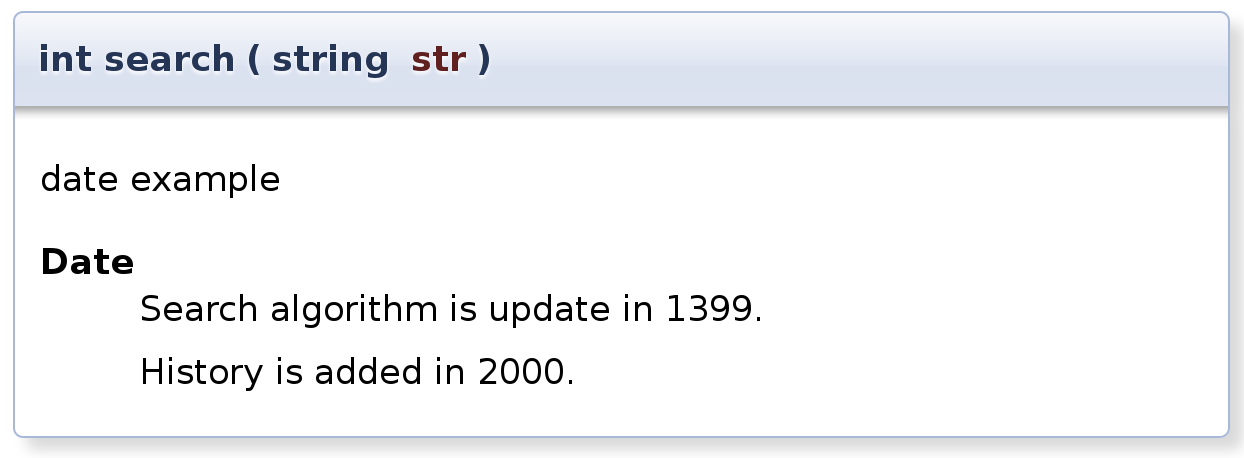
\includegraphics[width=0.8\textwidth]{image/write/document-the-code/developer-info/date-multi}
	\caption[چند برچسب تاریخ]{
		استفاده از چندین برچسب تاریخ پشت سر هم.
	}
	\label{write/document-the-code/developer-info/date-multi}
\end{figure}


\subsection{نسخه}
% version 
% \version { version number }

در پروژه‌های نرم‌افزاری، تغییراتی ایجاد شده در هر بسته با استفاده از یک شماره
مرز بندی می‌شود که به آن نسخه می‌گویند.
برای نمونه فرض کنید که در طول زمان چهار ویژگی به یک بسته نرم‌افزاری اضافه شده
است، یک مرزبندی این است که دو ویژگی در نسخه شماره ۱ و دو ویژگی دگر در نسخه شماره
۲ قرار گیرد.
در نسخه بندی یک سیستم، ترتیب صعودی میان نسخه‌ها به منزله پیشرفت پروژه در نظر
گرفته می‌شود.
در نمونه اورده شده نیز بعد از نسخه شماره ۲ تمام چهار ویژگی در سیستم وجود خواهد
داشت در حالی که نسخه شماره ۱ تنها شامل دو ویژگی است.
نسخه بندی یک سیستم و یا محصول بر اساس سیاست‌هایی است که در توسعه به کار می‌رود و
در حوزه این کتاب جای ندارد از این رو به آن نخواهیم پرداخت.

مستند فنی، به عنوان یک مستند جامع از یک سیستم باید شامل اطلاعاتی در زمینه نسخه
بندی و ویژگی‌های هر نسخه نیز باشد.
بر این اساس برچسب \lr{version} برای تشریح خصوصیت‌های یک نسخه در مستند فنی در نظر
گرفته شده است.
ساختار کلی این برچسب به صورت زیر است:
\begin{C++}
/**
 * \version { version number }
 */
\end{C++}

متن ورودی این برچسب می‌تواند به صورت یک پاراگراف کامل در نظر گرفته شود که شامل
توضیحات کامل در مورد این نسخه است.
در این متن می‌توان از تمام روش‌های زیباسازی متن و برچسب‌های نمایشی استفاده کرد.
پایان متن ورودی این برچسب با رسیدن به یک خط خالی و یا برچسب تعیین می‌شود.

\begin{note}
این برچسب برای تشریح امکانات، تغییرات و یا به روز رسانی‌هایی استفاده می‌شود و
می‌تواند برای هر موجودیت به صورت جداگانه به کار گرفته شود.
بهتر است از این برچسب زمانی استفاده شود که موجودیت مورد نظر شامل تغییرات و یا
شرایط جدید باشد.
\end{note}

امکان استفاده از این برچسب به صورت متوالی نیز فراهم شده است.
تمام برچسب‌هایی که به صورت متوالی آورده شده باشد، با یک دیگر ترکیب شده و در
خروجی نمایشد داده می‌شود.
توضیحات مربوط به هر نسخه در این حالت با شروع یک خط جدید در مستند نمایش داده شده
و یک خروجی مناسب را ایجاد می‌کند.
یک روش معادل نیز تشریح تمام تغییرات با استفاده از یک برچسب است که استفاده از این
روش توصیه نمی‌شود.


\subsection{نویسندگان}
% author
% \author { list of authors }
% \authors { list of authors }

نام نویسنده و یا نویسندگان، از دیگر اطلاعات توسعه است که در مستند فنی در نظر
گرفته می‌شود.
نام نویسنده و یا نویسندگان را با استفاده از برچسب \lr{author} تعیین می‌کنند که
در حالت کلی به صورت زیر است:
\begin{C++}
/**
 * \author {list of autohrs}
 */
\end{C++}

برای نمونه فرض کنید که یک تابع توسط سه نویسنده پیاده‌سازی شده است، در این صورت
مستند مربوط به این تابع، در حالت کلی، به صورت زیر خواهد بود:
\begin{C++}
/**
 * \brief author example
 *
 * \author author1
 * author2
 * author3
 */
int author(string str);
\end{C++}

مستند نهایی تولید شده برای این مستند در شکل
\ref{write/document-the-code/developer-info/author-multi} نمایش داده شده است.
فهرست نویسندگان، همانگونه در این نمونه قابل ملاحضه است، می‌تواند شامل چندین نام
باشد.
پاراگرافی که بعد از این برچسب نوشته شود به صورت کامل به عنوان پارامتر این برچسب
در نظر گرفته می‌شود.
این برچسب ساختار خاصی را برای پاراگراف ورودی در نظر نمی‌گیرد بنابر این می‌توان
از تمام برچسب‌های که در نمایش متن و زیبا سازی آن کاربرد دارد، استفاده کرد.
انتهای این برچسب با استفاده از یک خط خالی و یا آغاز یک بخش دیگر تعیین می‌شود.
\begin{figure}
	\centering
	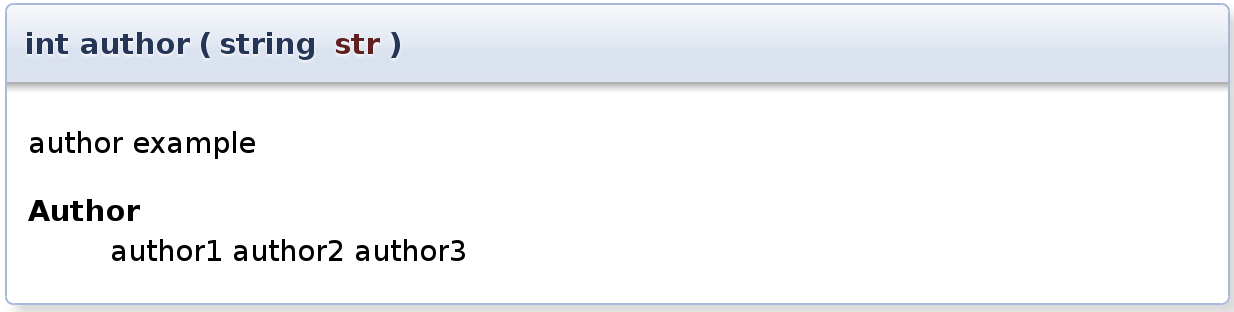
\includegraphics[width=0.8\textwidth]{image/write/document-the-code/developer-info/author-multi}
	\caption[فهرست نویسندگان]{
		فهرست نویسندگان.
	}
	\label{write/document-the-code/developer-info/author-multi}
\end{figure}


همانگونه که در نمونه بالا قابل مشاهده است، می‌توان فهرست تمام نویسندگان را با
استفاده از یک برچسب بیان کرد.
روش مناسب‌تر استفاده از این برچسب برای هر نویسنده است به این ترتیب نام
نویستنده‌گان هرکدام به صورت مستقل در یک خط نوشته می‌شود.
از این رو می‌توان نمونه بالا را به صورت زیر اصلاح کرد:
\begin{C++}
/**
 * \brief author example
 *
 * \author author1
 * \author author2
 * \author author3
 */
int author1(string str);
\end{C++}
مستند تولید شده برای این مستند در شکل \ref{write/document-the-code/developer-info/author-multi1}
نمایش داده شده است.
\begin{figure}
	\centering
	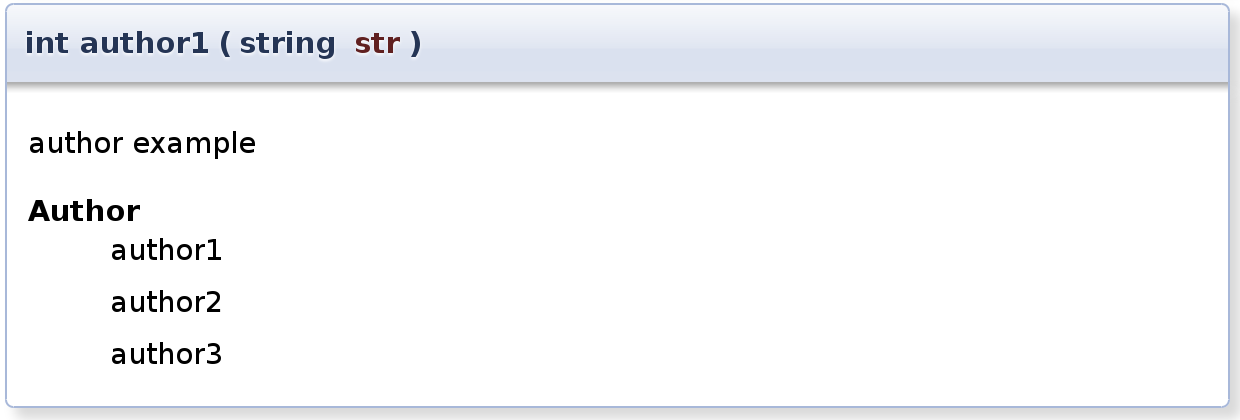
\includegraphics[width=0.8\textwidth]{image/write/document-the-code/developer-info/author-multi1}
	\caption[فهرست نویسندگان]{
		فهرست نویسندگان با به کاربردن چندین برچسب متوالی.
	}
	\label{write/document-the-code/developer-info/author-multi1}
\end{figure}

یک روش دیگر استفاده از برچسب \lr{authors} است.
تنها تفاوت میان این دو برچسب، عنوانی است که در خروجی تولید می‌شود.
با استفاده از برچسب \lr{authors} عنوان تولید شده در خروجی نیز به صورت جمع خواهد
بود در حالی که برچسب \lr{author} به صورت مفرد است.
به عنوان نمونه اصلاح نمونه بالا به صورت زیر مستند شکل
\ref{write/document-the-code/developer-info/author-multi2} را ایجاد می‌کند که
تنها در عنوان با یکدیگر متفاوت هستند.
\begin{C++}
/**
 * \brief author example
 *
 * \authors author1
 * \authors author2
 * \authors author3
 */
int authors(string str);
\end{C++}
\begin{figure}
	\centering
	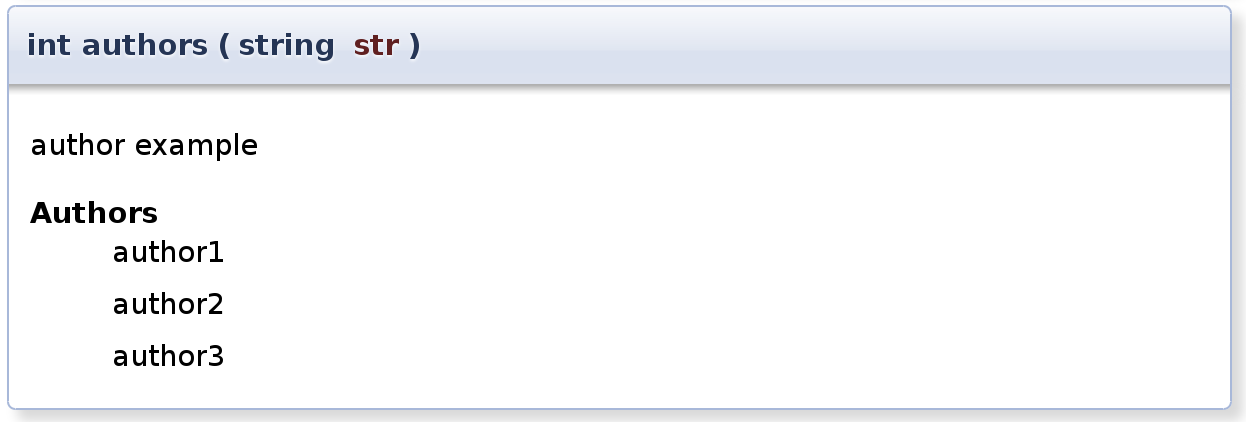
\includegraphics[width=0.8\textwidth]{image/write/document-the-code/developer-info/author-multi2}
	\caption[فهرست نویسندگان]{
		فهرست نویسندگان با استفاده از برچسب \lr{authors}.
	}
	\label{write/document-the-code/developer-info/author-multi2}
\end{figure}


\subsection{نسخه شروع}
% since
% \since { text }

در فرآیند توسعه سیستم‌ها، موجودیت‌های و امکانات متفاوت در برهه‌های زمانی و یا
نسخه‌های متفاوتی از سیستم ایجاد می‌شوند.
با استفاده از برچسب \lr{since} زمان اضافه شدن یک موجودیت به بسته اضافه تعیین می‌شود.
ساختار کلی این برچسب به صورت زیر است:
\begin{C++}
/**
 * \since { text }
 */
\end{C++}

در متن ورودی این برچسب، که در حالت کلی یک پاراگراف است، از ساختار خاصی استفاده نمی‌شود
و می‌توان تمام برچسب‌های زیباسازی متن را در آن به کار برد.
متن ورودی این برچسب با رسیدن به یک سطر خالی و یا برچسب‌های دیگر خاتمه می‌یابد.
برای نمونه فرض کنید که یک فراخوانی از نسخه ۲ یک بسته معرفی شده است، مستند مورد نیاز برای 
این فراخوانی، در ساده‌ترین حالت، به صورت زیر است:
\begin{C++}
/**
 * \brief since example
 *
 * \since 2.0.0 last update
 */
int since(string str);
\end{C++}

مستند ایجاد شده برای این نمونه در شکل \ref{write/document-the-code/developer-info/since} نمایش 
داده شده است.
\begin{figure}
	\centering
	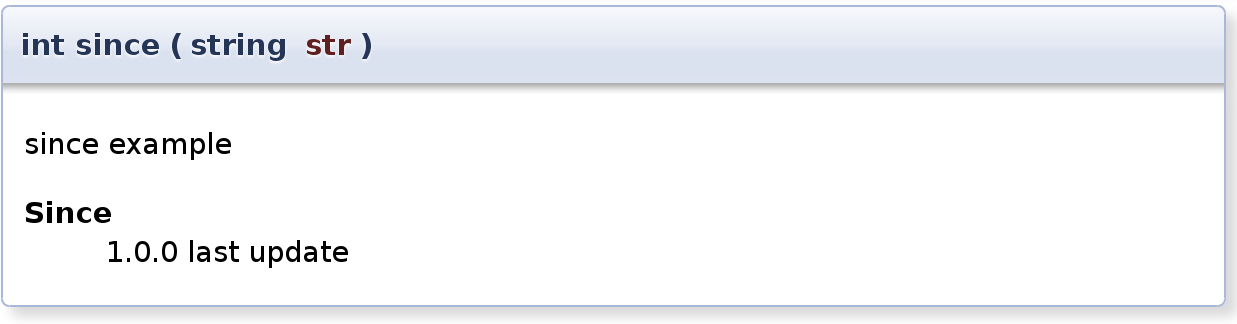
\includegraphics[width=0.8\textwidth]{write/document-the-code/developer-info/since}
	\caption[فهرست نویسندگان]{
		تعیین رویداد و یا نسخه‌ای اضافه شدن یک سیستم.
	}
	\label{write/document-the-code/developer-info/since}
\end{figure}

\begin{warning}
امکان استفاده از این برچسب بیش از یک بار برای هر موجودیت وجود دارد با این وجود این کار
از نظر مستند سازی کاملا اشتباه است.
ظهور یک امکان جدید تنها در یک زمان ممکن است و بعد از آن ممکن است دستخوش تغییراتی شده
و به روز شود.
برای نمایش تغییرات و به روز رسانی‌های از برچسب‌های دیگری مانند \lr{date}
\end{warning}

\subsection{کنارگذاشتن}
% deprecated
% \deprecated { description }

کنار گذاشتن و یا حذف یک امکان از سیستم در طول حیات آن بسیار معمول است.
در بسیاری از موارد امکانات ایجاد شده کارایی خود را از دست داده و یا با امکانات
جدید اضافه شده در تضاد هستند.
از این رو باید به ناچار آنها را کنار گذاشت و این موضوع را به نوعی به کاربران آن
سیستم انتقال داد.
اما سیستم‌ها باید به گونه‌ای توسعه یابند که با سازکارهای قدیم خود سازگار بوده و
سیستم‌های وابسته به خود را حمایت کنند.
نمی‌توان اینگونه تصور کرد که به محض کنار گذاشتن یک امکان از طراحی، در پیاده سازی
نیز باید آن را حذف کرد.

یک روش مناسب برای کنار گذاشتن یک امکان از سیستم، اعلام این کار در نسخه جاری و
اجرای آن در نسخه‌های آینده است.
در این روش امکان مورد نظر به صورت یک امکان کنار گذاشته معرفی می‌شود و در مستند
فنی به کاربران سیستم اعلام می‌شود.
در نهایت بعد از چند نسخه، بنا بر سیاست‌های توسعه، امکان مورد نظر به صورت کامل
حذف می‌شود.
در مستند سازی فنی از برچسب \lr{depricated} برای تعیین امکاناتی استفاده می‌شود که
در حال حاضر کنار گذاشته شده و در آینده نیز به صورت کامل از سیستم حذف می‌شود.
ساختار کلی این برچسب به صورت زیر است:
\begin{C++}
/**
 * \deprecated {description }
 */
\end{C++} 

از این برچسب برای تشریح ورش‌های جایگزین، زمان انقضا و حذف کامل و یا هر مستند
مورد نیاز برای موجودیت و یا امکان کنارگذاشته شده، استفاده می‌شود.
برای نمونه فرض کنید که یک فراخوانی در سیستم در نظر گرفته شده بوده است و در
طراحی به این نتیجه رسیده‌ایم که این فراخوانی باید حذف شود.
حداقل مستند مورد نیاز برای این فراخوانی به صورت زیر است:
\begin{C++}
/**
 * \brief deprecated example
 *
 * \deprecated This method will be removed in V2.0.1 completely, please use
 * deprecated2(string) instead.
 */
int deprecated(string str);
\end{C++}

در شکل \ref{write/document-the-code/developer-info/deprecated} خروجی تولید شده
برای این مستند نمایش داده شده است.
در فرآیند تولید مستند فنی، تمام موجودیت‌هایی که به عنوان یک موجودیت کنارگذاشته
شده تعیین می‌شوند در یک فهرست جمع آورده شده و به مستند اضافه می‌شود.
به این ترتیب با ارائه شدن یک نسخه جدید از سیستم و مستند فنی آن، کاربران
می‌توانند به سادگی فهرست تمام امکانات کنارگذاشته شده را مشاهده و تغییرهای مورد
نیاز را در سیستم‌های خود ایجاد کنند.
در شکل \ref{write/document-the-code/developer-info/deprecated-list} یک نمونه از
فهرست موجودیت‌های کنارگذاشده شده آورده شده است.
\begin{figure}
	\centering
	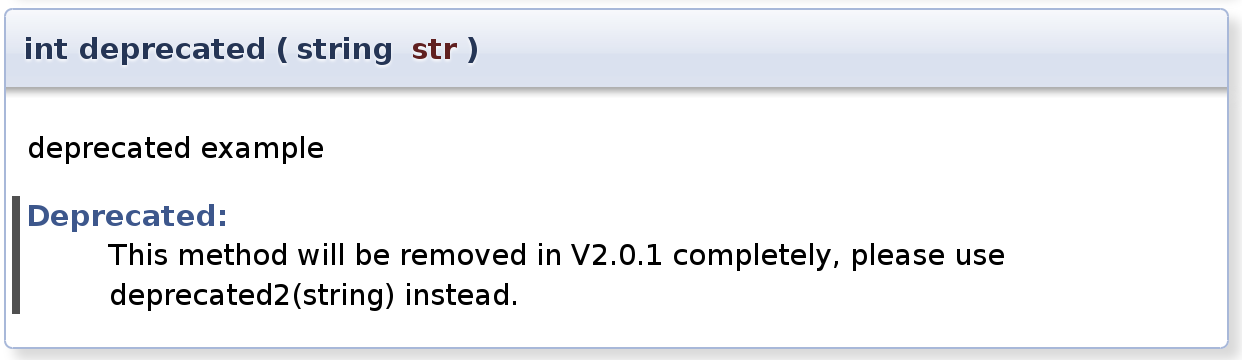
\includegraphics[width=0.8\textwidth]{image/write/document-the-code/developer-info/deprecated}
	\caption[موجودیت کنار گذاشته شده]{
		مستند یک موجودیت کنار گذاشته شده. در این مستند نه تنها روش جایگزین بلکه زمان
		حذف کامل این موجودیت نیز بیان شده است.
	}
	\label{write/document-the-code/developer-info/deprecated}
\end{figure}
\begin{figure}
	\centering
	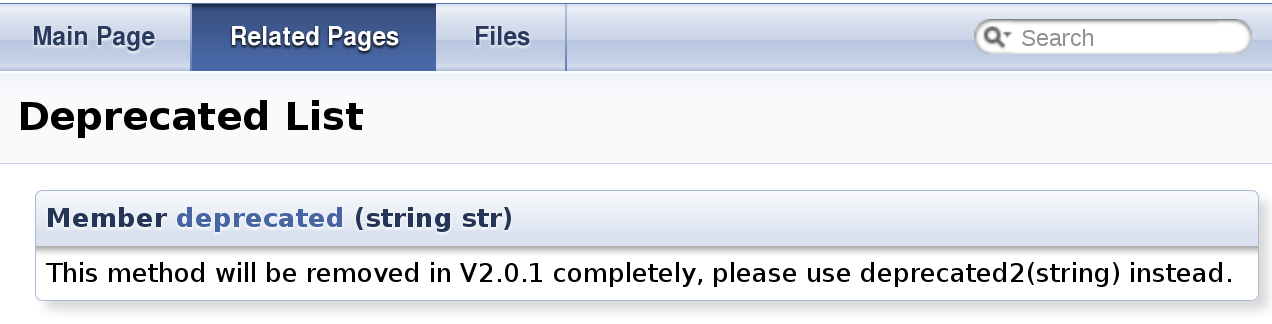
\includegraphics[width=0.8\textwidth]{write/document-the-code/developer-info/deprecated-list}
	\caption[فهرست موجودیت‌های کنار گذاشته شده]{
		فهرست تمام موجودیت‌های حذف شده. این فهرست کاربران را در توسعه و تغییر سیستم‌های خود
		یاری می‌کند.
	}
	\label{write/document-the-code/developer-info/deprecated-list}
\end{figure}


% \subsection{بخش}
% remarker
% \remark { remark text }
% 
% Starts a paragraph where one or more remarks may be entered. The paragraph will
% be indented. The text of the paragraph has no special internal structure. All
% visual enhancement commands may be used inside the paragraph. Multiple adjacent
% \remark commands will be joined into a single paragraph. Each remark will start
% on a new line. Alternatively, one \remark command may mention several remarks.
% The \remark command ends when a blank line or some other sectioning command is
% encountered.




\section{مستند توابع}

تابع‌ها یکی از پایه‌ای ترین موجودیت‌ها در زبان‌های برنامه سازی هستند.
پیدایش تابع مصادف با ارائه شدن راهکارهای برنامه سازی به صورت پیمانه‌ای بوده است.
امروزه تقریبا تمام زبان‌های برنامه‌سازی عمومی مبتنی بر توابع طراحی و پیاده سازی
می‌شوند.
در مستند نویسی نیز نگاهی ویژه به این موجودیت وجود دارد.
در مستند فنی برچسب‌ها و راهکارهای متفاوتی برای مستند سازی این موجودیت ارائه شده
است که در این بخش به بررسی این موارد خواهیم پرداخت.

\subsection{پارامترها}
% param
% \param [(dir)] <parameter-name> { parameter description }

پارامترهای ورودی و خروجی مهم‌ترین خصوصیت از یک تابع است که در مستند فنی باید به آن پرداخته شود.
برای توصیف پارامترها تابع برچسب \lr{param} در نظر گرفته شده است.
مستند فنی پارامترها انقدر مهم است که در فرآیند تولید مستند فنی، پارامترهای بدون مستند کشف شده و 
به صورت اخطار نمایش داده می شود.
ساختار کلی این برچسب به صورت زیر است:
\begin{C++}
\param [(dir)] <parameter-name> { parameter description }
\end{C++}

اولین پارامتر این برچسب جهت پارامتر را برای تابع تعیین می‌کند.
اگر پارامتر یک پارامتر ورودی برای تابع باشد با \lr{in} و اگر پارامتر
به عنوان خروجی تابع در نظر گرفته شده باشد با \lr{out} نمایش داده می‌شود.
برای پارامترهایی که در یک تابع به عنوان ورودی و خروجی به کار می‌روند، هر دو مقدار 
با هم به کار می‌رود.
در نمونه زیر هر سه حالت ممکن برای جهت پارامترها وجود دارد. 
\begin{C++}
/**
 * \brief Function argument example
 *
 * \param[in]      param1 First argument.
 * \param[out]      param2 Second argument.
 * \param[in,out] param3 Third argument.
 */
int param(string param1, int* param2, double* param3);
\end{C++}

پارامتر دوم نام پارامتر و پاراگراف بعد از آن توصیف پارامتر است. در شکل
\ref{write/document-the-code/function/param} مستند تولید شده برای نمونه
بالا آورده شده است.
\begin{figure}
	\centering
	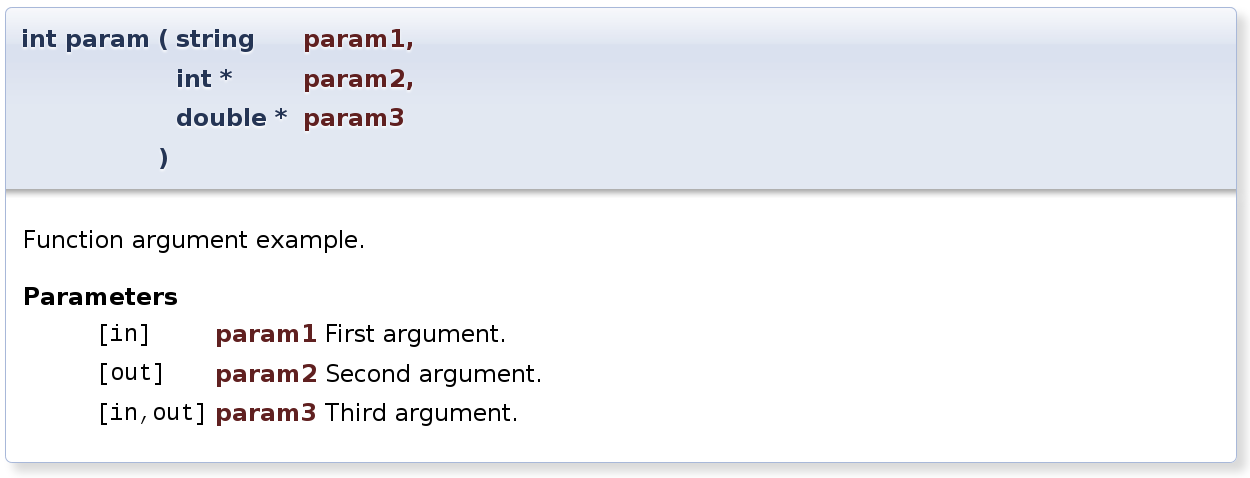
\includegraphics[width=0.8\textwidth]{write/document-the-code/function/param}
	\caption[پارامترهای یک تابع]{
		پارامترهای یک تابع.
	}
	\label{write/document-the-code/function/param}
\end{figure}

توصیف پارامتر ورودی از ساختار خاصی پیروی نمی‌کند و می‌تواند شامل تمام دستورهای
زیبا سازی متن باشد.
تمام برچسب‌های \lr{param} که پست سر هم قرار می‌گیرند با هم ادغام شده و به صورت یک 
بخش مستقل در مستند ظاهر می‌شوند.
در این بخش مستند توصیف هر پارامتر از یک خط جدید آغاز می‌شود.
شروع یک برچسب و یا بخش دیگر انتهای توصیف این برچسب را تعیین می‌کند.

در بسیاری از موارد چندین پارامتر برای نمایش یک موجودیت به کار گرفته می‌شوند.
برای نمونه یک نقطه در فضای سه بعدی با استفاده از سه عدد نمایش داده می‌شود.
در این حالت می‌توان نام چندین پارامتر را به صورت هم زمان به عنوان ورودی نام 
برای این برچسب به کار برد.
نام پارامترها در این حالت با استفاده از کاما از یکدیگر جدا می‌شود.
در زیر یک نمونه آورده شده است که در آن سه پارامتر با هم مستند شده است.
مستند تولید شده برای این نمونه نیز در شکل 
\ref{write/document-the-code/function/param-multi-with-single-tag} نمایش داده شده است.
\begin{C++}
/**
 * \brief Multiple parameter with single param tag.
 * \param x,y,z Coordinates of the position in 3D space.
 * \param t     Time of event.
 */
void param2(double x,double y,double z,double t);
\end{C++}

\begin{figure}
	\centering
	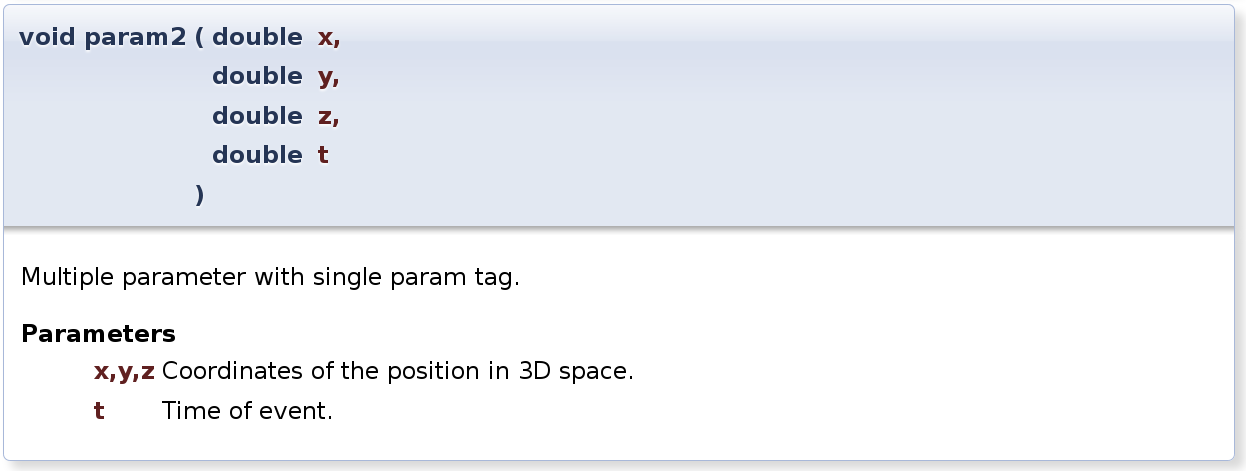
\includegraphics[width=0.8\textwidth]{write/document-the-code/function/param-multi-with-single-tag}
	\caption[پارامترهای یک تابع]{
		پارامترهای یک تابع. زمانی که چندین پارامتر برای یک کار مشترک به کار گرفته می‌شود
		می‌توان تمام آنها را به صورت یکجا مستند کرد. در این نمونه یک نقطه سه بعدی با سه 
		عدد صحیح نمایش داده شده است و در مستند فنی هر سه با هم مستند شده.
	}
	\label{write/document-the-code/function/param-multi-with-single-tag}
\end{figure}



\subsection{خروجی}
% return
% \return { description of the return value }

در اغلب زبان‌های برنامه سازی همه منظوره، یک نوع داده به عنوان نوع داده خروجی تابع
در نظر گرفته می‌شود.
در مستند سازی فنی برچسب \lr{return} برای مستند کردن خروجی تابع در نظر گرفته شده است.
ساختار کلی استفاده از این برچسب به صورت زیر است:
\begin{C++}
\return { description of the return value }
\end{C++}

ساختار متن توصیف خروجی یک تابع، از ساختار خاصی پیروی نمی‌کند و می‌تواند شامل
انواع برچسب‌های زیبا سازی متن باشد.
بر خلاف اینکه بسیاری از زبانهای مشهور مانند \lr{java}، \lr{C/C++} و \lr{C\#} تنها از 
یک نوع داده خروجی حمایت می‌کنند، امکان استفاده مکرر از این برچسب نیز وجود دارد.
در فرآیند تولید مستند فنی، تمام برچسب‌های \lr{return} که به صورت متوالی ظاهر شده‌اند
با یکدیگر ترکیب شده و در یک بخش نمایش داده می‌شوند.
متن توصیف خروجی تابع با شروع بخش جدید و یا یک برچسب دیگر، پایان می‌یابد.

در \lr{Doxygen} یک برچسب دیگر به نام \lr{returns} برای تشریح خروجی‌های یک تابع در نظر گرفته شده است.
از این برچسب زمانی استفاده می‌شود که بیش از یک خروجی برای یک تابع در نظر گرفته شده است.
ساختار کلی این برچسب به صورت زیر است:
\begin{C++}
\returns { description of the return value }
\end{C++}

\begin{note}
برچسب \lr{returns} کاملا شبیه به \lr{return} است و ویژگی خاصی ندارد. 
زمانی که تعداد خروجی‌های بیش از یکی باشد این برچسب مستند زیباتر و قابل درکی را 
ایجاد می‌کند.
\end{note}

\subsection{استثناها}
% throw
% exception
% \exception <exception-object> { exception description }

با ظهور زبان‌های برنامه سازی، راهکارهایی برای مدیریت خطا پیشنهاد شد که در آن
یک تابع خطا را تولید یک خروجی خاص نمایش می‌داد.
این نوع خروجی را \glspl{exception} می‌نامند که در زبان‌های برنامه سازی راهکاری متفاوت
از خروجی‌های معمولی را برای آنها در نظر می‌گیرند.
نکته‌ای که در مستند سازی فنی باید به آن توجه داشت این است که تمام استثناهای یک
تابع باید به صورت کامل مستند شود.
برای مستند کردن \glspl{exception} از برچسب \lr{exception} استفاده می‌شود.
ساختار کلی این برچسب به صورت زیر است:
\begin{C++}
\exception <exception-object> { exception description }
\end{C++}

دو پارامتر ورودی برای این برچسب در نظر گرفته شده که به ترتیب نام و توصیف استثنا
است.
وجود یک استثنا در یک تابع بررسی نمی‌شود از این رو مستند ساز باید در
مستند کردن استثنا دقت کند.
پاراگراف توصیف استثنا از ساختار خاصی پیروی نمی‌کند و می‌توان از برچسب‌های دیگر مانند
برچسب‌های زیبا سازی متن در آن استفاده کرد.
متن توصیف یک استثنا با رسیدن به یک خط خالی، بخش جدید و یا برچسب دیگر پایان می‌پذیرد.

معمولا توابع انواع متفاوتی استثنا تولید می‌کنند که هر یک حالت خاصی را نمایش می‌دهد.
از این رو امکان استفاده از چندین برچسب \lr{exception} فراهم شده است.
در فرآیند تولید مستند فنی، برچسب‌هایی که به صورت متوالی ظاهر شده‌اند با هم ترکیب
شده و در یک بخش نمایش داده می‌شوند.
در این حالت توصیف هر استثنا با شروع یک خط جدید آغاز می‌شود.
در نمونه زیر تابعی با دو نوع استثنا متفاوت مستند شده است و خروجی معادل با آن در شکل 
\ref{write/document-the-code/function/exception} نمایش داده شده است.
\begin{C++}
/**
 * \brief exception explanation
 *
 * \exception Exp1 Exception should be discussed here.
 * \exception Exp2 Exception should be discussed here.
 * \exception Exp3 Exception should be discussed here.
 *
 * This section causes new exception section to be generated by Doxygen.
 *
 * \exception Exp4 Exception should be discussed here.
 * \exception Exp5 Exception should be discussed here.
 */
int excetpion(Param p1, Param p2);
\end{C++} 
\begin{figure}
	\centering
	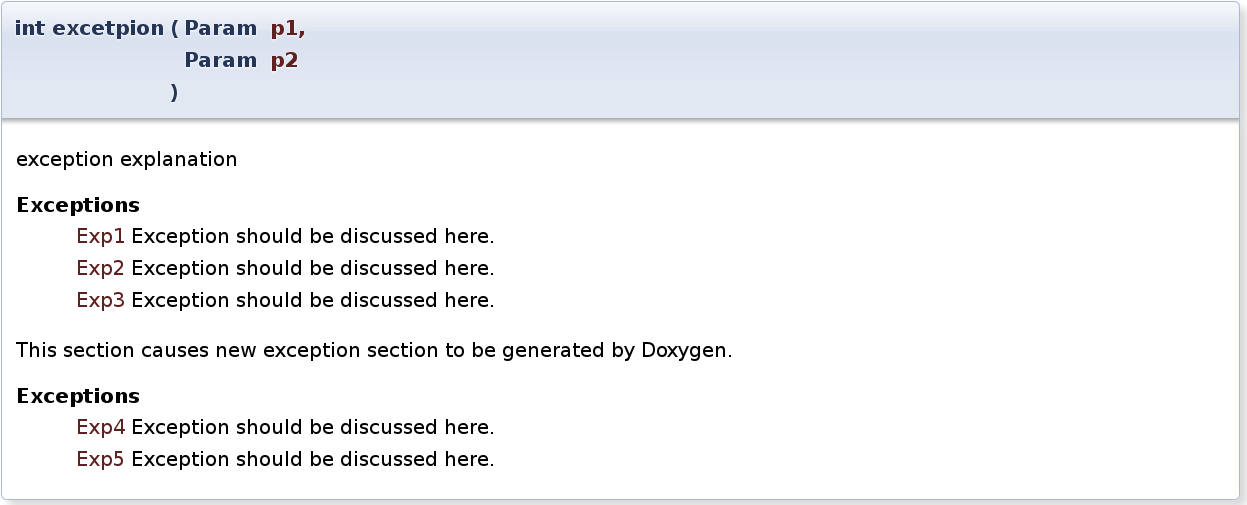
\includegraphics[width=0.8\textwidth]{image/write/document-the-code/function/exception}
	\caption[استثناهای یک تابع]{
		برچسب‌های \lr{exception} که به صورت پشت سر هم اورده شده است با یک دیگر ترکیب شده 
		و در یک بخش نمایش داده می‌شود.
	}
	\label{write/document-the-code/function/exception}
\end{figure}

برخی از ابزارهای مستند سازی از برچسب \lr{throw} برای توصیف یک استثنا استفاده می‌شود.
شاید دلیل این کار کلمه ذخیره شده \lr{throw} است که برای تولید یک استثنا در برخی
از زبان‌های برنامه سازی مانند \lr{C++} و \lr{java} استفاده می‌شود.
در \lr{Doxygen} نیز از این برچسب حمایت می‌شود.
ساختار کلی این برچسب به صورت زیر است:
\begin{C++}
\throw <exception-object> { exception description }
\end{C++}

زمانی که تعداد استثناها بیش از یکی باشد، می‌توان از برچسب \lr{throws} نیز استفاده کرد.

% TODO: maso 1392: پیش نیاز و پس نیاز یک تابع
% \subsection{پیش نیاز و پس نیاز}
% \post { description of the postcondition }
% 
% Starts a paragraph where the postcondition of an entity can be described. The
% paragraph will be indented. The text of the paragraph has no special internal
% structure. All visual enhancement commands may be used inside the paragraph.
% Multiple adjacent \post commands will be joined into a single paragraph. Each
% postcondition will start on a new line. Alternatively, one \post command may
% mention several postconditions. The \post command ends when a blank line or some
% other sectioning command is encountered.
% 
% \pre { description of the precondition }
% 
% Starts a paragraph where the precondition of an entity can be described. The
% paragraph will be indented. The text of the paragraph has no special internal
% structure. All visual enhancement commands may be used inside the paragraph.
% Multiple adjacent \pre commands will be joined into a single paragraph. Each
% precondition will start on a new line. Alternatively, one \pre command may
% mention several preconditions. The \pre command ends when a blank line or some
% other sectioning command is encountered.


% TODO: maso 1392: گراف فراخوانی یک تابع
% \subsection{گراف فراخوانی}
% callgraph
% callergraph
% \callgraph
% 
% When this command is put in a comment block of a function or method and HAVE_DOT
% is set to YES, then doxygen will generate a call graph for that function
% (provided the implementation of the function or method calls other documented
% functions). The call graph will be generated regardless of the value of
% CALL_GRAPH.
% 
% Note
%     The completeness (and correctness) of the call graph depends on the doxygen
%     code parser which is not perfect.
% 
% See Also
%     section \callergraph.
% 
% \callergraph
% 
% When this command is put in a comment block of a function or method and HAVE_DOT
% is set to YES, then doxygen will generate a caller graph for that function
% (provided the implementation of the function or method calls other documented
% functions). The caller graph will be generated regardless of the value of
% CALLER_GRAPH.
% 
% Note
%     The completeness (and correctness) of the caller graph depends on the
%     doxygen code parser which is not perfect.
% 
% See Also
%     section \callgraph.









% 
\section{محیط‌های خاص}


note

warning

bug

todo

attention

brief

detail

verbatin

test

code


% %
% حق نشر 1390-1402 دانش پژوهان ققنوس
% حقوق این اثر محفوظ است.
% 
% استفاده مجدد از متن و یا نتایج این اثر در هر شکل غیر قانونی است مگر اینکه متن حق
% نشر بالا در ابتدای تمامی مستندهای و یا برنامه‌های به دست آمده از این اثر
% بازنویسی شود. این کار باید برای تمامی مستندها، متنهای تبلیغاتی برنامه‌های
% کاربردی و سایر مواردی که از این اثر به دست می‌آید مندرج شده و در قسمت تقدیر از
% صاحب این اثر نام برده شود.
% 
% نام گروه دانش پژوهان ققنوس ممکن است در محصولات دست آمده شده از این اثر درج
% نشود که در این حالت با مطالبی که در بالا اورده شده در تضاد نیست. برای اطلاع
% بیشتر در مورد حق نشر آدرس زیر مراجعه کنید:
% 
% http://dpq.co.ir/licence
%
\section{مدیریت مستندها}

if

copycode

copybrief

copydetail

include

includehtml

htmlonly

xmlonly

latexonly

manonly


% %
% حق نشر 1390-1402 دانش پژوهان ققنوس
% حقوق این اثر محفوظ است.
% 
% استفاده مجدد از متن و یا نتایج این اثر در هر شکل غیر قانونی است مگر اینکه متن حق
% نشر بالا در ابتدای تمامی مستندهای و یا برنامه‌های به دست آمده از این اثر
% بازنویسی شود. این کار باید برای تمامی مستندها، متنهای تبلیغاتی برنامه‌های
% کاربردی و سایر مواردی که از این اثر به دست می‌آید مندرج شده و در قسمت تقدیر از
% صاحب این اثر نام برده شود.
% 
% نام گروه دانش پژوهان ققنوس ممکن است در محصولات دست آمده شده از این اثر درج
% نشود که در این حالت با مطالبی که در بالا اورده شده در تضاد نیست. برای اطلاع
% بیشتر در مورد حق نشر آدرس زیر مراجعه کنید:
% 
% http://dpq.co.ir/licence
%
\section{پیوند}


می‌توان با استفاده از دستورهای متفاوت منابع را بیان کرد. پیوند میان مستندها را
ایجاد کرد. از این میان می‌توان به موارد زیر اشاره کرد:

ref

cite

ancher

see

sa

link


